\chapter{مروری بر کارهای پیشین}
\newpage
‎\renewcommand{\baselinestretch}{2}\normalsize‎
\label{Previous works_2}
در این فصل، پس از بیان یک مقدمه در زمینه فاکتورهای موثر بر کارآیی و همگرایی الگوریتم‌های یادگیری توزیع‌شده، راه‌حل‌های ارائه شده برای یادگیری توزیع‌شده، الگوریتم‌های یادگیری توزیع‌شده انتشاری و نقاط ضعف راه‌حل‌های موجود مرور خواهند شد. 

\section{مقدمه}
امروزه با افزایش حجم داده‌های پردازشی و همچنین نیاز به انجام محاسبات سنگین در بسیاری از حوزه‌ها، راه‌کارهای بسیاری برای پیاده‌سازی الگوریتم‌های توزیع‌شده به منظور تسریع فرآیند یادگیری و بهبود نرخ همگرایی ارائه شده است. انتخاب پلتفرم مناسب برای پیاده‌سازی یکی از مواردی است که تاثیر بسیار زیادی بر کارآیی الگوریتم دارد. الگوريتم‌هاي موازي بر روي پلتفرم‌هاي 1) سيستم حافظه اشتراكي (\lr{multi-core } يا \lr{many-core}) 2) سیستم حافظه اشتراکی توزیع‌شده 3) سیستم حافظه توزیع‌شده یا شبكه كامپيوتري پياده‌سازي می‌شوند \cite{lian2019}. هر یک از پلتفرم‌ها مزایا، کاربردها و معایبی دارند. 

مورد دیگر، مدل‌های محاسباتی موازی هستند که تاثیر بسیاری بر همگام‌سازي گره‌ها و کارایی الگوریتم‌ها دارند و هم روشی مفید برای هدایت طراحان الگوریتم‌های موازی و برنامه‌نویسان برای بهینه‌سازی کد و بهره‌برداری از ویژگی‌های سخت‌افزاری جدید ارائه می‌دهند. همچنین در حوزه سیستم‌های یادگیری توزیع‌شده به منظور تسریع عملیات و مدیریت بهتر بخش‌های مختلف محاسبات و ارتباطات و همچنین همگام‌سازي مناسب گره‌ها، پیاده‌سازی فرآیند یادگیری توزیع‌شده باید تحت یک مدل محاسباتی موازی از جمله  \lr{PRAM}، \lr{LogP}، \lr{BSP} و \lr{MapReduce} انجام شود. مدل محاسباتی \lr{PRAM} یک مدل حافظه اشتراکی است و به دلیل محدودیت در تعداد پردازنده‌ها و بالا بودن هزینه ارتباطات نسبت به هزینه محاسبات برای پیاده‌سازی همه جانبه مناسب نیست. مدل محاسباتی \lr{LogP} مدل برنامه‌نویسی ندارد و ارتباطات پردازنده‌ها در آن به صورت یک نمای محلی بر اساس عملکرد هر جفت پردازنده است. در مقاله \cite{BSP2012} تفاوت‌های بین چارچوب نگاشت-کاهش و مدل محاسباتی \lr{BSP} مورد بحث قرار گرفته‌اند و این واقعیت برجسته شده است که الگوریتم‌های \lr{BSP} به دلیل نیاز به ذخیره‌سازی و دسترسی به داده‌ها در چندین ابرگام، در صورتی که تعداد ابرگام‌ها ثابت نباشد، نمی‌توانند به طور موثر با استفاده از چهارچوب نگاشت-کاهش پیاده‌سازی شوند. این مورد به دلیل ماهیت چارچوب نگاست-کاهش است که اجازه ذخیره‌سازی داده بین دورها را نمی‌دهد، اما الگوریتم‌های \lr{BSP} مستلزم این هستند که به این داده‌ها بین چنین دورهایی دسترسی داشته باشند. همچنین، آنها نشان دادند که مدل \lr{BSP} می‌تواند برای مدل‌سازی الگوریتم‌های نگاشت-کاهش با هزینه جانبی یکسان برای سیستم‌های معمولی با تعداد پردازنده‌های یکسان استفاده شود. بنابراین، مشخص شده است که \lr{MapReduce} باید صرفاً به عنوان یک چارچوب پیاده‌سازی با \lr{BSP} برای طراحی الگوریتم‌ها استفاده شود. با این حال، برای کارهایی با زمان اجرا ناشناخته، \lr{MapReduce} همچنان باید استفاده شود زیرا \lr{BSP} دارای قابلیت تعادل بار پویا نیست. به عنوان مثال، فریمورک محاسبات توزیع‌شده\lr{Apache hama} از مدل \lr{BSP} استفاده می‌کند و گره‌ها می‌توانند با یکدیگر ارتباط برقرار کنند، در حالیکه فریمورک \lr{Apache Hadoop} مبتنی بر چارچوب نگاشت-کاهش است و گره‌ها در انتهای هر دور تنها  مجاز به ارتباط با پردازنده مرکزی هستند. 

مورد سوم، پیاده‌سازی الگوریتم‌های یادگیری توزیع‌شده به صورت متمرکز و غیرمتمرکز است. روش متمرکز یک الگوی پیاده‌سازی است که که در آن تعداد زیادی از گره‌ها با یک یا چند سرور مرکزی هماهنگ می‌شوند تا یک مدل را بدون به اشتراک گذاشتن داده‌های اولیه و خام خود یاد بگیرند. گره‌ها داده‌های میانی از جمله گرادیان‌ها، بردارهای تخمین‌زده و غیره را به سرورهای مرکزی ارسال می‌کنند و با استفاده از نتایج میانگین‌گیری شده دریافتی از سرورها ادامه محاسبات خود را انجام می‌دهند. در این نوع پیاده‌سازی چنین تبادلات داده‌ای دائما بین گره‌ها و سرورهای مرکزی انجام می‌شود. روش غیرمتمرکز الگوی پیاده‌سازی دیگری برای ماشین‌های یادگیری توزیع‌شده  بدون حضور سرور مرکزی است که هر گره بعد از انجام محاسبات محلی، داده‌های میانی خویش را با یک یا تعدادی گره همسایه دیگر تبادل کرده و ادامه محاسبات را بر اساس داده‌های دریافتی انجام می‌دهد. در الگوریتم‌های یادگیری توزیع‌شده غیرمتمرکز  استراتژی‌های متفاوتی برای انتخاب گره‌های همسایه ارائه شده است. 

مورد موثر چهارم بر کارایی الگوریتم‌های یادگیری توزیع‌شده، روش همگام‌سازي یا مکانیزم کنترل مانع بین گره‌ها است.  در حال حاضر، روش‌های کنترل مانع را می‌توان به طور کلی به سه مکانیزم موازی غیرهمگام \footnote{\lr{Asynchronous Parallel}} (\lr{ASP})، مکانیزم موازی همگام با کهنگی \footnote{\lr{Stale Synchronous Parallel}}(\lr{SSP}) و مکانیزم موازی همگام مانعی \footnote{\lr{Bulk Synchronous Parallel}} (\lr{BSP}) دسته‌بندی کرد \cite{NIPS2012}. مکانیزم \lr{BSP} یک طرح قطعی است که در آن گره‌ها یک مرحله محاسباتی را انجام می‌دهند و به دنبال آن یک مرحله همگام‌سازی یا ارتباطات برای تبادل به‌روزرسانی‌ها را انجام می‌دهند. این روش اطمینان می‌دهد از طریق جلوگیری از رفتن هر گره به مرحله بعدی تا زمانی که همه گره‌ها بتوانند محاسبات را به اتمام برسانند، همه گره‌ها در یک تکرار محاسباتی یکسانی قرار خواهند داشت. علاوه بر این، اثرات محاسبات فعلی برای گره‌ها تا زمانی که مانع انجام نشده است، قابل مشاهده نیست. با توجه به اینکه تضمین‌های صحت برنامه سریال برای برنامه‌های \lr{BSP} اغلب قابل تحقق است، در نتیجه \lr{BSP} قوی‌ترین روش کنترل مانع خواهد بود \cite{Ho2013}. متأسفانه \lr{BSP} یک نقطه ضعف بزرگ دارد. از آنجایی که گره‌ها باید منتظر بمانند تا کار دیگران به پایان برسد، در صورت وجود گره‌هایی با قدرت محاسباتی کمتر در یک شبکه ناهمگن \cite{NIPS2012} و یا گره‌هایی که به دلیل عوامل تصادفی و غیرقابل پیش‌بینی به زمان بیشتری برای تکمیل یک مرحله نیاز دارند، کارایی محاسبات در این مدل براساس کندترین ماشین تعیین می‌گردد. این امر منجر به کاهش چشمگیر عملکرد سیستم می‌شود. به طور کلی، \lr{BSP} دقت محاسباتی بالایی دارد اما در محیط‌های ناهمگن از کارایی پایین رنج می‌برد.

مکانیزم \lr{ASP} ساده‌ترین مدل است که هیچ همگام‌سازی بین گره‌ها رخ نمی‌دهد. این مکانیزم نقطه متقابل مکانیزم کنترل مانع \lr{BSP} است و اجازه می‌دهد محاسبات با حداکثر سرعت ممکن از طریق اجرای کاملا غیرهمگام گره‌ها انجام شود. در محیط‌های محاسباتی همگن، که در آن گره‌ها پیکربندی‌ مشابهی دارند، مکانیزم \lr{ASP} هم‌گرایی سریعی دارد و بالاترین توان عملیاتی تکرار را نتیجه می‌دهد. اما در حالت کلی، این غیرهمگامی باعث تاخیر در به‌روزرسانی و اعمال نویز و خطا در محاسبات می‌شود. در نتیجه، مکانیزم \lr{ASP} از کاهش کیفیت تکرار رنج می برد و حتی ممکن است در برخی از محیط‌ها واگرا شود. به طور کلی، \lr{ASP} سرعت‌های بسیار خوبی را در همگرایی ارائه می‌دهد، اما خطر واگرایی بیشتری به خصوص در محیط‌های ناهمگن دارد.

مکانیزم \lr{SSP} یک مدل همگام محدود شده است که می‌تواند به عنوان یک مدل \lr{BSP} سست شده در نظر گرفته شود. به‌جای اینکه همه گره‌ها را ملزم کند در یک تکرار باشند، سیستم تصمیم می‌گیرد که آیا گره ممکن است بر اساس میزان عقب‌تر بودن از کندترین گره، (یک کهنگی محدود از پیش تعریف‌شده) کار کند. به طور خاص، گره‌ای که بیش از \lr{s } تکرار از سریعترین گره عقب باشد، خیلی کند در نظر گرفته می‌شود. اگر چنین گره‌ای وجود داشته باشد، سیستم گره‌های سریع‌تر را متوقف می‌کند تا زمانی که گره کند به آنها برسد. این \lr{s} به عنوان پارامتر کهنگی شناخته می‌شود. این پارامتر به مکانیزم \lr{SSP} اجازه می‌دهد تا همگرایی قطعی را تضمین کند \cite{Ho2013}. به عبارت‌ دیگر، این مکانیزم تفاوت تعداد تکرارها بین سریعترین و کندترین گره‌ها را کنترل می‌کند و با مجبور کردن سریعترین گره به صبر تا زمانی‌که از آستانه فراتر نرود، آن را در محدوده آستانه قرار می‌دهد. مکانیزم \lr{SSP} یک راه‌حل کوتاه‌بینانه ارائه می‌دهد، زیرا ظرفیت محاسباتی هر گره (یعنی سرعت آن) را در نظر نمی‌گیرد و فقط به تعداد تکرارهایی که هر گره انجام داده است ، توجه می‌کند. به طور کلی، مکانیزم \lr{SSP} مصالحه خوبی بین \lr{BSP} کاملاً قطعی و همگام و \lr{ASP} کاملاً غیرهمگام ارائه می‌کند. با تنظیم پارامتر کهنگی $s = 0 $ در \lr{SSP}، روش \lr{BSP} را خواهیم داشت. درحالی‌که با تنظیم $s=\infty$ مکانیزم \lr{ASP} اجرا می‌شود. شکل \ref{p26} یک مقایسه کلی از سه مکانیزم کنترل مانع بر اساس میزان سازگاری (سرعت همگرایی) و سرعت (بازده) یادگیری، به تصویر کشیده است. 

\begin{figure}
	\begin{center}
		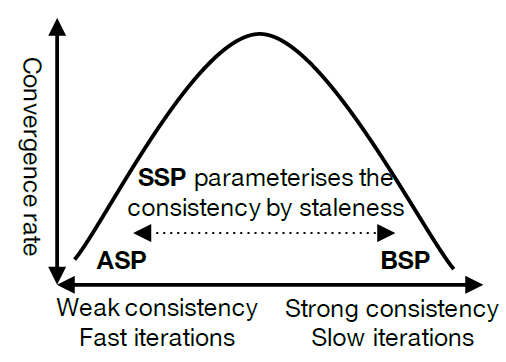
\includegraphics[scale=0.6]{Pic26.png}
		\caption{مقایسه سه مکانیزم کنترل مانع \cite{Zhao2021}}
		\label{p26}
	\end{center}
\end{figure}

به طور خلاصه در شکل \ref{Barrier} تکنیک‌های همگام‌سازی و کنترل مانع که تا کنون معرفی شده‌اند به همراه تکنیک کنترل مانع پیشنهادی در این رساله به نام تکنیک همگام منطقه‌ای \lr{FBSP} آورده شده است. تکنیک غیرهمگام احتمالی \lr{PSP} نیز در بخش \ref{CmpMld} به عنوان یک راه‌کار مبتنی بر مدل محاسباتی متمرکز تشریح خواهد شد.

\begin{figure}
	\begin{center}
		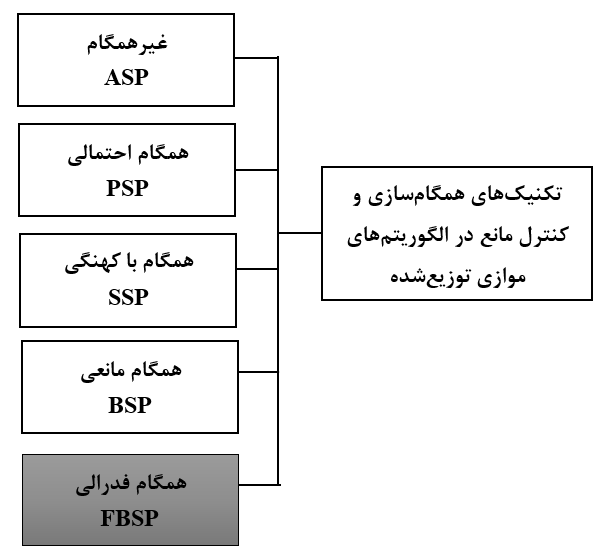
\includegraphics[scale=1.2]{BarrierTypes_.PNG}
		\caption{مکانیزم‌های کنترل مانع موجود و مکانیزم پیشنهادی در این رساله}
		\label{Barrier}
	\end{center}
\end{figure}

\section{بیان راه‌حل‌های موجود برای یادگیری توزیع‌شده}

در سیستم‌های حافظه اشتراکی همه پردازنده‌ها به یک حافظه مشترک دسترسی دارند و از نظر سخت‌افزاری همه پردازنده‌ها از طریق یک گذرگاه به حافظه فیزیکی مشترک دسترسی دارند. این پردازنده‌ها می‌توانند به طور مستقل کار کنند در حالی که همه آنها به یک حافظه دسترسی دارند. هر گونه تغییر در متغیرهای ذخیره شده در حافظه توسط همه پردازنده‌ها قابل مشاهده است. در صورتی که پردازنده $i$ در حال استفاده از یک متغیر باشد و به طور هم‌زمان پردازنده $j$ با دسترسی به همان متغیر بر روی آن تغییری اعمال نماید، در واقع پردازنده $i$ با نسخه قدیمی آن متغیر کار می‌کند. این سیستم‌ها از مشکل خواندن‌های ناسازگار رنج می‌برند. اكثر الگوریتم‌های موازی مطرح شده در سیستم‌های حافظه اشتراکی نیاز به همگام‌سازي پردازنده‌ها و يا قفل‌کردن برای کنترل دسترسی هم‌زمان پردازنده‌ها به حافظه اشتراکی دارند. این موارد سبب پایین آمدن کارایی طرح‌ها و الگوریتم‌های موازی مي‌شود. با توجه به اینکه قفل‌های نرم‌افزاری هزینه‌های بسیار زیادی دارند، در حالت ایده‌آل طرحی مناسب است که بدون انتظار و قفل باشد. 
در نوعی دیگر از سیستم‌های حافظه که با نام ماشین‌های دسترسی حافظه غیریکنواخت \lr{NUMA}\footnote{\lr{Non-Uniform Memory Access}} یا سیستم‌های حافظه اشتراکی توزیع‌شده شناخته می‌شوند، تعدادی پردازنده \lr{CPU} با هسته‌های بسیار وجود دارد که زمان دسترسی به حافظه توسط هر پردازنده کاملا بستگی به مکان قرار گرفتن حافظه نسبت به آن دارد. یک پردازنده می‌تواند به حافظه محلی خود سریعتر از حافظه غیرمحلی (حافظه محلی پردازنده دیگر یا حافظه مشترک بین پردازنده‌ها) دسترسی پیدا کند. بزرگترین مزیت \lr{NUMA} انتقال سریع داده‌ها و تاخیر کمتر در سیستم‌های چندپردازشی است؛ بنابراین این سیستم‌ها برای برنامه‌های بلادرنگ و حیاتی به کار می‌روند.
در سیستم‌های حافظه توزیع‌شده هر پردازنده حافظه محلی خود را دارد و پردازنده‌ها از طریق یک شبکه با هم در ارتباط هستند. به عبارتی، حافظه توزیع‌شده در مفهوم سخت‌افزاری به حالتی اطلاق می‌شود که پردازنده‌ها فقط می‌توانند حافظه محلی خود را مستقیما ببیند و تنها از طریق شبکه می‌توانند به حافظه پردازنده‌های دیگر دسترسی داشته باشند. در این مدل سیستم‌ها انواع مختلف پردازنده‌ها را می‌توان تجربه کرد.

الگوریتم‌های ارائه شده برای یادگیری توزیع‌شده بر روی پلتفرم‌هاي حافظه اشتراکی، حافظه اشتراکی توزیع‌شده \lr{NUMA} و حافظه توزیع‌شده پیاده‌سازی شده‌اند. در شکل \ref{Cat1} دسته‌بندی راه‌حل‌های ارائه شده برای یادگیری توزیع‌شده براساس چهار دیدگاه مختلف انجام شده است: 1) نوع سیستم حافظه اشتراکی/توزیع‌شده، 2) استفاده/عدم استفاده از مدل محاسباتی، 3) متمرکز/غیرمتمرکز بودن و 4) همگام/غیرهمگام بودن مکانیزم کنترل مانع. در شکل \ref{Cat1} جایگاه رویکرد پیشنهادی \lr{FBSP} در این رساله نیز نشان داده شده است. 

 \begin{figure}
	\begin{center}
		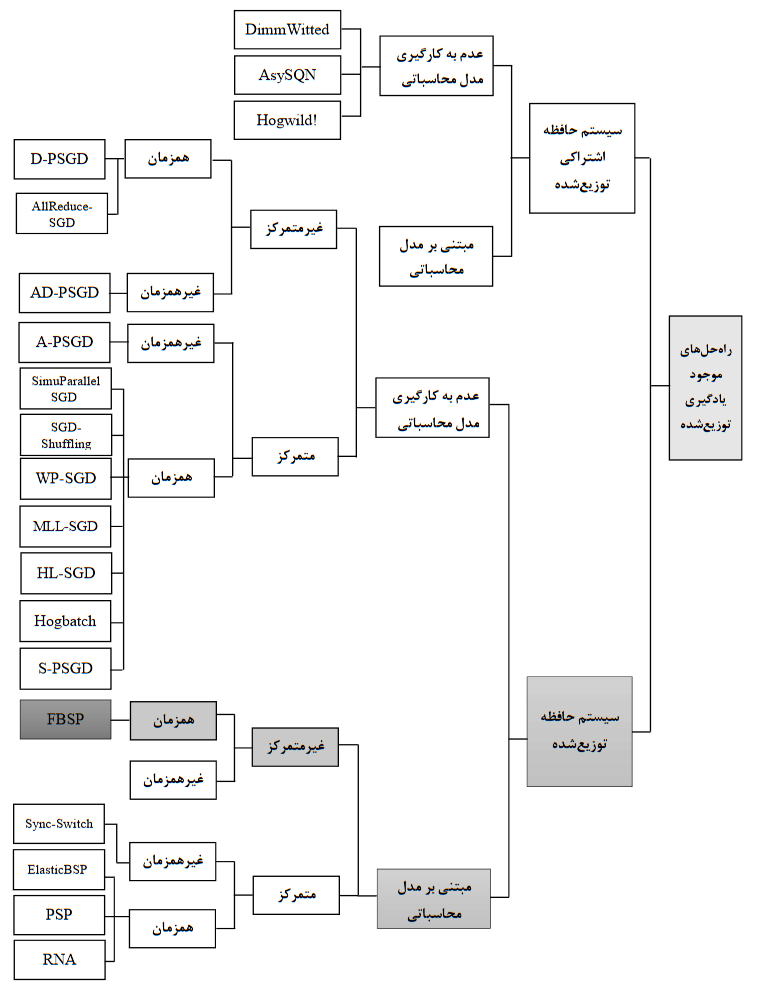
\includegraphics[scale=1.2]{CatApprochs_1.PNG}
		\caption{دسته‌بندی راه‌حل‌های موجود برای یادگیری توزیع‌شده}
		\label{Cat1}
	\end{center}
\end{figure}

در بخش‌های \ref{WthCmpMdl} و \ref{CmpMld} راه‌حل‌های ارائه شده در حوزه یادگیری توزیع‌شده با جزئیات بیشتری شرح داده خواهند شد.  هر یک از راه‌حل‌های معرفی شده در این دو بخش از الگوریتم یادگیری یا به عبارتی روش به‌روزرساني متفاوتی در فرآیند یادگیری خویش بهره می‌گیرد. در سال‌های اخیر، الگوریتم‌های انتشار بر روی شبکه‌های تطبیقی توزیع‌شده به دلیل همگرایی سریع و رسیدن به میانگین خطا کمتر در حالت پایدار و همچنین مقیاس‌پذیری، غیرمتمرکز بودن و مقاومت این نوع شبکه‌ها در برابر خرابی گره‌ها و یال‌ها بسیار مورد توجه محققان قرار گرفته‌اند. شبکه‌های تطبیقی توزیع‌شده برای یادگیری مجموعه داده‌های بزرگ با بهره‌مندی از قدرت همکاری میان گره‌ها مناسب می‌باشند. در بخش \ref{DfsnAlg} الگوریتم‌های یادگیری تطبیقی انتشار معرفی‌شده مورد بررسی قرار می‌گیرند و یک دسته‌بندی از آنها نیز ارائه می‌گردد.

\subsection{راه‌حل‌های توزیع‌شده بدون مدل محاسباتی}\label{WthCmpMdl}


در \cite{Hog12011} یک استراتژی ساده برای اجرای \lr{SGD} به صورت موازی و بدون قفل به نام \lr{Hogwild! } ارائه شده است که پردازنده‌ها (گره‌ها) اجازه دسترسی یکسان به حافظه اشتراکی را دارند و می‌توانند اجزای مجزای حافظه را به دلخواه خود به‌روزرسانی کنند. از آنجایی که پردازنده‌ها می‌توانند تغییرات پردازنده‌های دیگر را بازنویسی کنند، الگوریتم بدون قفل ممکن است دچار مشکل شود. در این مقاله نشان داده شده است که وقتی دسترسی به داده‌ها به صورت خلوت  باشد یا به عبارتی در هر گام فقط بخش کوچکی از بردار پارامتر به‌روزرسانی شود، بازنویسی حافظه توسط پردازنده‌های مختلف به ندرت رخ می‌دهد و در صورت بروز در محاسبات خطا دیده خواهد شد. در این استراتژی یک تسریع تقریبا خطی با توجه به تعداد پردازنده‌ها برای مسائل یادگیری خلوت از نظر تئوری و تجربی ارائه شده است اما همان طور که بیان شد تنها برای مسائل بهينه‌سازي خلوت قابل اعمال است. تابع هزینه خلوت در استراتژی \lr{Hogwild!} به صورت زیر تعریف می‌شود:

\begin{equation}\label{e18}
	f(w)=\sum_{e\in E}f_e(w,x_e)
\end{equation}

که بردار پارامتر $w$ در حافظه اشتراكي ذخيره می‌شود و توسط تمام پردازنده‌ها در دسترس است. $e$ زیرمجموعه کوچکی از $\{1, 2, ...,M\}$ است و $x_e$ مقادير بردار ورودی $x$ با توجه به نقاط انتخاب شده در $e$ را نشان می‌دهد.

در مقاله \cite{Zin2010} یک الگوریتم \lr{SGD} موازی بر اساس یک استراتژی تک-میانگین‌گیری  به نام \lr{SimuParallel SGD } ارائه شده است و مبنا را بر مدل داده-موازی گذاشته است. به عبارتی \lr{m } نمونه داده بین \lr{k} پردازنده تقسیم شده و در هر تکرار $t$ هر پردازنده \lr{i} به صورت مستقل و بدون هیچ تبادل و همکاری با دیگر پردازنده‌ها، گرادیان کاهشی تصادفی را با توجه به داده‌ $c^{i,t}$ و بردار پارامتر $w_{i,t}$ محاسبه می‌کند. زمانی که اجرای تمام پردازنده‌ها به پایان رسید، در نقطه همگام‌سازی نتایج تجمیع و سپس میانگین آنها به عنوان نتیجه نهایی در نظر گرفته می‌شود.

الگوریتم گرادیان کاهشی تصادفی موازی همگام\footnote{\lr{Synchronous Parallel Stochastic Gradient Descent (S-PSGD)}}  \lr{(S-PSGD)} یک روش یادگیری توزیع‌شده موازی است که در مقاله \cite{Mini2016} برای حل توابع هزینه غیرمحدب و در \cite{dekel2012} برای حل توابع هزینه محدب معرفی شده است. پیاده‌سازی این الگوریتم به صورت متمرکز و با حضور یک سرور پارامتر  \footnote{\lr{Parameter server}} انجام شده است. در هر گام هر گره بردار پارامتر را از سرور پارامتر خوانده و گرادیان تصادفی دسته‌ای را محاسبه می‌کند. سپس گره‌ها گرادیان‌های خود را به سرور پارامتر ارسال کرده و بعد از همگام‌سازی، با استفاده از میانگین گرادیان‌ها بردار پارامتر ذخیره‌شده در سرور پارامتر به‌روزرسانی می‌شود. به دلیل وجود گام همگام‌سازی، اکثر گره‌ها باید در حالت انتظار قرار بگیرند تا کار آهسته‌ترین گره به اتمام برسد. در این روش هزینه گام‌ همگام‌سازی $O(N)$ است. زمانی که $N$ بزرگ باشد، سبب هزینه‌های ارتباطی بالا در سرور پارامتر می‌شود. 

در مقاله \cite{nccl} برای پیاده‌سازی الگوریتم \lr{AllReduce-SGD } از قانون به روزرسانی دقیقاً مشابه \lr{S-PSGD} در هر تکرار استفاده شده است. هیچ سرور پارامتری در این الگوریتم وجود ندارد. گره‌ها با یک شبکه حلقه بهم متصل شده‌اند و هر گره نسخه محلی از مدل را نگه می‌دارد. در هر تکرار، هر گره گرادیان دسته‌ای را محاسبه کرده و سپس از \lr{AllReduce} برای همگام‌سازی گرادیان‌ها استفاده می‌کنند. در نهایت هر گره میانگین همه گرادیان‌ها را بدست می‌آورد. این الگوریتم در شبکه‌ای با تاخیر بالا کند عمل خواهد کرد. در پایان تکرار، مدل محلی هر گره با میانگین گرادیان‌ها به‌روز می‌شود. به دلیل وجود همگام‌سازی در هر تکرار، زمان بیکاری همانند الگوریتم \lr{S-PSGD} بالا است. 

ماشین‌های  \lr{NUMA}\footnote{\lr{Non-Uniform Memory Access}} از تعدادی پردازنده \lr{CPU} با هسته‌های زیاد تشکیل شده‌اند. به عبارت دیگر مدلی از طراحی سخت‌افزاری است که در سرورهایی با چند \lr{CPU} استفاده می‌شود و استفاده از حافظه توسط یک پردازنده \lr{CPU} کاملا بستگی به مکان قرار گرفتن حافظه نسبت به آن دارد. استراتژی  \lr{DimmWitted} \cite{DimmWitted} یک تحلیل آماری بر روی روش‌های تکثیر مدل و داده و همچنین شیوه‌های دسترسی به داده‌ها در حافظه اصلی يك ماشين \lr{NUMA} ارائه داده است. در واقع گره‌ها بر روی گره‌های یک ماشین \lr{NUMA} پیاده‌سازی شده‌اند و همگام‌سازي مدل‌ها بر روي گره‌ها انجام می‌شود. این همگام‌سازی تا زمانی‌ که مانع عبور و مرور داده‌ها در حافظه اصلی نشود، سودمند است. به منظور همگام‌سازی در این استراتژی، یک نخ در هر گره به صورت متناوب مدل‌های روی تمام گره‌ها را می‌خواند و پس از میانگین‌گیری نتایج، کپی مدل ‌در گره را به‌روزرسانی می‌‌کند.

در مقاله \cite{lian2019} با استفاده از دو پلتفرم حافظه اشتراکی و شبکه کامپیوتری (حافظه توزیع‌شده) دو الگوریتم \lr{SGD} توزیع‌شده موازی غیرهمگام\footnote{\lr{Asynchronous}} به صورت متمرکز برای حل مسائل بهینه‌سازی غیرمحدب معرفی شده است. این الگوریتم با نام \lr{A-PSGD } شناخته شده‌است که در مقاله \cite{ag2011} از این الگوریتم برای حل مسائل محدب نیز استفاده شده است. در الگوریتم \lr{AsySG-con} \cite{lian2019} که بر روی پلتفرم شبکه‌ کامپیوتری پیاده‌سازی شده است، بردار پارامترها بر روی سرور مرکزی قرار دارد و در طول گام به‌روزرسانی، گره‌ها اجازه دسترسی به بردار پارمترها را ندارند. در نتیجه فرآیند خواندن بردار سازگار خواهد بود. برای ایجاد ارتباط بین گره‌ها و سرور مرکزی از کتابخانه \lr{MPICH} کمک گرفته شده است. برای پياده‌سازي الگوریتم‌های غيرهمگام، از یک پارامتر کهنگی\footnote{\lr{Staleness}}  استفاده می‌شود و مقادير قديمي بردار پارامتر براي ارزيابي گراديان تصادفي سایر گره‌ها به‌کار گرفته می‌شود. هر گره داده‌های نمونه را به صورت دسته‌های \lr{M}تایی تصادفی دریافت کرده و پس از محاسبه گرادیان آن را به سرور مرکزی ارسال می‌کند. سرور مرکزی با قبول یک میزان کهنگی $\tau _{k,m}$ در پارامترهای دریافتی از گره‌های شبکه به‌روزرسانی بردار پارامتر $w_{k+1}$ را انجام می‌دهد. 

\begin{equation}\label{e23}
	w_{k+1}=w_k-{\gamma}_k \sum_{m=1}^{M}G(x_{k-\tau_{k,m}},\xi_{k,m})
\end{equation}

میزان کهنگی گرادیان‌های دریافتی از گره نباید از یک حدی بیشتر باشد. زیرا همگرایی الگوریتم را به شدت کاهش می‌دهد و در بعضی مواقع سبب واگرایی آن می‌شود. براي داشتن همگرايي مناسب، میزان کهنگی نبايد زياد بزرگ باشد و یک حدآستانه‌ به صورت $\max_{k,m} \tau _{k,m}\le T$ در نظرگرفته شود \cite{Avron2014}.

در الگوریتم \lr{AsySG-INcon} \cite{lian2019} که بر روی پلتفرم حافظه اشتراکی پیاده‌سازی شده است، بردار پارامتر \lr{w} بر روی حافظه اشتراکی قرار می‌گیرد و هر گره بردار پارامتر را از حافظه خوانده و در حافظه محلی خود قرار می‌دهد و با استفاده از داده‌های نمونه و $\hat{w ̂}$ (مقدار خوانده شده از حافظه اشتراکی)  مقدار گرادیان $G(\hat{w}_k;\xi_k)$ را به صورت محلی محاسبه می‌کند. سپس بردار پارامتر $w$ در حافظه اشتراکی بدون قفل نرم‌افزاری به صورت زیر به‌روزرسانی می‌شود.
\begin{equation}\label{e24}
	(w_{k+1})_{i_k}=(w_k)_{i_k}-\gamma \sum_{m=1}^{M}(G(\hat{w}_{k,m},\xi_{k,m}))_{i_k} 
\end{equation}

که $i_k\in \{{1,2,…,M}\}$ یک اندیس تصادفی انتخاب شده برای به‌روزرسانی توسط گره \lr{k} و \lr{n} طول بردار پارامتر را نشان می‌دهد. الگوریتم \lr{A-PSGD } بر روی حافظه اشتراکی از مشکل خواندن‌های ناسازگار رنج می‌برد. راه‌حل استفاده شده برای غلبه بر این مشکل برگرفته از روش ارائه شده در \cite{Avron2014} می‌باشد. با مانیتور کردن مقدار بردار پارامتر در حافظه اشتراکی و استفاده از تعریف  $w_k$ به صورت زیر تا حدی این مشکل را می‌توان برطرف کرد:
\begin{equation}\label{e25}
	\hat{w}_k=w_k-\sum_{j\in J(k)} (w_{j+1}-w_j) 
\end{equation}

\begin{equation}\label{e26}
	J(k)\subset {k-1,...,k-T}, \quad \lvert J(k)\rvert\le T
\end{equation}

مجموعه $J(k)$ در رابطه \ref{e26} برای مانیتور کردن مقدار بردار پارامتر  در حداکثر $T$ گره دیگر است. 

زمانی‌که شرایط شبکه مساعد باشد، روش‌های \lr{SGD} موازی توزیع‌شده تسریع مشابه‌ای خواهند داشت و تفاوت این روش‌ها زمانی مشخص می‌شود که شبکه‌ای با پهنای باند کم و در نتیجه تاخیر بالا داشته باشیم. در الگوریتم \lr{D-PSGD} \cite{Lian20171} با حذف سرور مرکز سعی شده است یک \lr{SGD} موازی غیرمتمرکز همگام برای کاهش بار ترافیکی سرور و برطرف کردن معایب الگوریتم‌های قبلی معرفی شود. یکی از معایب این الگوریتم هزینه بالای همگام‌سازی گره‌ها در شبکه است. برای توزیع دادها می‌توان کل داده‌ها را در اختیار همه گره‌ها قرار داد یا داده‌ها را به شکلی مناسب پارتیشن‌بندی کرد و هر پارتیشن را در اختیار یک گره قرار داد. برای پیاده‌سازی این الگوریتم از چارچوب‌کاری یادگیری عمیق ماکروسافت \lr{CNTK} و کتابخانه \lr{Torch} استفاده شده است. 

در مقاله \cite{lian2018} الگوریتم غیرمتمرکز غیرهمگام  \lr{AD-PSGD } برای یادگیری موازی توزیع‌شده معرفی شده و معایب رویکردهای قبلی را برطرف کرده است. برای هر گره \lr{i} یک نخ محاسباتی (برای انجام محاسبات گرادیان‌ها و به‌روزرسانی وزن‌ها) و یک نخ ارتباطی (برای برقرار ارتباط بین گره \lr{i} و یک همسایه تصادفی و ترکیب بردار وزن‌ آنها) با یک بافر مشترک \lr{g} تعریف شده است که به ترتیب بر روی \lr{GPU} و \lr{CPU} اجرا می‌شوند. پردازنده‌های \lr{GPU} به طور پيوسته گراديان‌ها را محاسبه و نتايج را بدون توجه به اينكه ميانگين‌گيري رخ مي‌دهد يا خير، در بافر پردازنده‌های \lr{CPU} قرار مي‌دهند. در این مقاله گره‌ها به دو دسته فعال و غیرفعال تقسیم می‌شوند. به منظور جلوگیری از بن‌بست در تبادل و میانگین‌گیری بردارهای پارامتر دو گره انتخاب‌ می‌شود، به طوریکه یک گره فعال همسایه‌اش را تنها از مجموعه گره‌های غیرفعال می‌تواند انتخاب کند. به منظور مدیریت فرآیند یادگیری غیرهمگام از یک تکنیک کهنگی استفاده شده است. 

در صورتی‌که گره‌های شرکت‌کننده در فرایند یادگیری توزیع‌شده از لحاظ قدرت محاسباتی و پردازشی با یکدیگر متفاوت باشند، پردازنده‌ها با عملکرد پایین تاثیر منفی بر نتیجه نهایی خواهند گذاشت. در \cite{WP2020} یک الگوریتم گرادیان کاهشی موازی وزن‌دار به نام \lr{WP-SGD } معرفی شده است که بردارهای پارامتر گره‌ها به صورت وزن‌دار برای تولید نتیجه نهایی با یکدیگر ترکیب می‌شوند. وزن اختصاص داده شده به بردار پارامتر هر گره بر اساس تاخیر بین آن و سریع‌ترین گره تعریف شده است.

در مقاله \cite{Ma2019} دو روش موازی‌سازی \lr{SGD} همگام و \lr{SGD} غیرهمگام با استفاده از معماری‌های‌ محاسباتی مختلف در یک سیستم واحد پیاده‌سازی شدند و تاثير آنها بر روي كارايي سخت افزاري و زمان همگرايي در حالت‌هاي مختلف داده و توابع زیان متفاوت مورد بررسي قرار گرفته است. آن‌ها به این نتیجه دست یافتن که انتخاب بين نوع معماری محاسباتی و روش به‌روزرسانی مدل  به نوع کار و ويژگي داده‌ها وابسته است. در روش \lr{SGD} همگام، يك نخ مسئول به‌روزرساني مدل است. اين روش سبب محدود شدن اجراي موازي داخل الگوریتم مي‌شود. بهترین انتخاب برای موازی‌سازی عبارت جبرخطي، گراديان تابع زیان در مرحله محاسبه گراديان می‌باشد که براي تسريع محاسبات، پياده‌سازي‌هاي موازي كارا از كتابخانه‌هاي جبرخطي بهينه‌شده همچون کتابخانه \lr{ViennaCL} استفاده مي‌شود. این کتابخانه هم برای داده‌های خلوت و هم داده‌های متراکم کاربرد دارد. در صورتی‌که کتابخانه تنسورفلو و دیگر چهارچوب‌های کاری یادگیری عمیق تنها داده‌های متراکم را پشتیبانی می‌کنند و نمی‌توانند مدل‌های با ابعاد خیلی بالا را مدیریت کنند. 

یک الگوریتم \lr{SGD} توزیع‌شده بر اساس روش‌های بُرزدن محلی\footnote{\lr{Local shuffling}}  و سراسری\footnote{\lr{Global shuffling}}  با استفاده از یک گره مرکزی در مقاله \cite{MENG201946} ارائه شده است. بُرزدن یکی از روش‌های رایج پردازش داده است که برای حل مسائل بزرگ یادگیری ماشین از تقسیم‌بندی داده‌ها در طول چندین ماشین یا نخ کاربرد دارد. در الگوریتم ارائه شده، داده‌های آموزشی برزده می‌شوند و سپس داده‌ها به صورت زیرمجموعه‌های غیرهمپوشان تقسیم شده و هر زیرمجموعه به یک گره اختصاص می‌یابد. بعد از انجام فرآیند یادگیری در هر تکرار، مجددا بُرزدن به صورت محلی یا سراسری انجام می‌شود. اگر بُرزدن به صورت سراسری باشد، بعد از بُرزدن داده‌ها مجدد در هر تکرار تقسیم‌بندی داده‌های آموزشی به صورت زیرمجموعه‌های غیرهمپوشان انجام می‌شود اما اگر بُرزدن به صورت محلی انجام شود، دیگر نیازی به تقسیم‌بندی مجدد داده‌های آموزشی نیست. نویسندگان مقاله نشان دادند که اگر عملیات بُرزدن مستقل باشد، بُرزدن سراسری معادل نمونه‌گیری بدون جایگزینی است و آن‌ها همگرایی الگوریتم \lr{SGD} توزیع‌شده به روش بُرزدن محلی و سراسری را برای مسائل غیرمحدب اثبات کردند. نرخ همگرایی برای بُرزدن محلی کندتر از بُرزدن سراسری است، زیرا اگر ارتباطی بین داده‌های تقسیم شده وجود نداشته باشد، برخی اطلاعات را از دست خواهیم داد.

الگوریتم مرتبه دوم \lr{AsySQN} \cite{tong2020} یک الگوریتم موازی غیرهمگام براساس روش شبه نیوتن تصادفی است که مبتنی بر یک پلتفرم حافظه اشتراکی برای حل مسائل بدشرط ارائه شده است. در الگوریتم \lr{AsySQN} براساس تکنیک‌های حافظه مدرن، از قفل‌هایی استفاده می‌شود که تضمین می‌کند در هر لحظه فقط یک پردازنده می‌تواند در حافظه اشتراکی بنویسد. بدین منظور یک تایمر سراسری \lr{t} بکار گرفته می‌شود و زمان‌های به‌روزرسانی حافظه اشتراکی را ذخیره می‌کند. در الگوریتم غیرهمگام، هنگامی‌که یک پردازنده در حال به‌روزرسانی پارامتر مشترک \lr{x} به $x_t$ است، پردازنده دیگر هنوز وضعیت قدیمی پارامتر $x_{D(t)}$ برای به روزرسانی و محاسباتش استفاده می‌کند. در اینجا $D(t)\in [t]$ حالت خاصی از پارامتر مشترک \lr{x} برای یک رشته یا پردازنده در زمانی است که $x$ در زمان $t$  به‌روز شده است. به منظور حفظ کارایی روش، حداکثر تاخیر بین فرآیندها به صورت $t-D(t)\le \tau$ محدود شده است. رابطه به‌روزرسانی استفاده شده در این روش در رابطه \ref{e22} بیان شده است.
\begin{equation}\label{e22}
	x_{t+1}=x_t-\eta H(x_{\hat{D}(t)})\nu(x_{\hat{D}(t)})
\end{equation}

از آنجایی که قدرت محاسباتی گره‌های شبکه ممکن است متفاوت باشد، با هدف افزایش نرخ همگرایی و استفاده بهینه از منابع در دسترس به طور هم‌زمان، در مقاله \cite{Ma2021} یک الگوریتم‌ \lr{SGD} توزیع‌شده با اندازه‌‌ دسته داده‌های سازگار  مبتنی بر معماری‌های ناهمگن \lr{CPU+GPU}  پیشنهاد شده است. میزان داده‌های اختصاص‌یافته به هر گره توسط یک گره هماهنگ‌کننده \footnote{\lr{Coordinator node}} به صورت پویا و تطبیقی در زمان اجرا و براساس سرعت پردازش آن گره تعیین می‌شود. 

در یک کار متفاوت \cite{Pu2021}، مساله بهینه‌سازی توزیع‌شده بر روی گراف‌های متغیر با زمان در نظر گرفته‌ شده است و یک الگوریتم ردیابی گرادیان تصادفی توزیع‌شده (\lr{DSGT})\footnote{\lr{Distributed stochastic gradient tracking algorithm}}  با معرفی متغیر کمکی $y_i$  برای هر گره به منظور ردیابی میانگین گرادیان تصادفی توابع هزینه را با فرض در دسترس بودن اطلاعات گرادیان دقیق، ارائه شده‌ است. در مرجع \cite{time2017} نیز روشی مشابه ارائه شده است. روش دیگری در این مقاله  \cite{Pu2021} به نام ردیابی گرادیان تصادفی شایعه (\lr{GSGT})  پیشنهاد شده است که براساس پروتکل‌های ارتباطی مبتنی بر \lr{Gossip} بوده و برای کاهش هزینه‌های ارتباطی در محاسبات توزیع‌شده کاربرد دارد. در هر تکرار یک گره‌ $i_k\in k$ به صورت تصادفی با احتمال $\frac{1}{n}$ فعال شده و با یکی از همسایه‌های خود $j_k$ با احتمال $\pi_{i_k j_k}$ ارتباط برقرار می‌کند و یا با احتمال $\pi_{i_k i_k}=1-\sum_{j\in N_{i_k}}\pi_{i_k j_k}$  با خودش به‌روز می‌شود. گام به‌روزرسانی هر گره $i$ به صورت زیر می‌باشد:

\begin{equation}\label{e27}
	\begin{cases}
		w_{i,k+1}=\frac{1}{2}(w_{i_k,k}+w_{j_k,k})-\alpha y_{i_k,k}\\
		y_{i,k+1}=\frac{1}{2}(y_{i_k,k}+y_{j_k,k})+g_i(w_{i,k+1},\xi_{i,k+1})-g_i(w_{i,k},\xi_{i,k})
	\end{cases}
\end{equation}

رویکرد‌های موازی و توزیع‌شده‌ای که اخیرا مبتنی بر الگوریتم گرادیان کاهشی ارائه شده‌اند، از لحاظ ویژگی‌هایی مانند پیچیدگی ارتباطی، زمان بیکاری یا معطلی و پلتفرم موازی استفاده‌شده در جدول \ref{Compare_Table} لیست شده‌اند. معیار پیچیدگی ارتباطی در جدول بر اساس نسبت $\frac{n_t}{n_h}$ تعریف شده است. که $n_t$ تعداد گرادیان‌ها یا مدل‌های انتقال‌داده‌ شده در پرمشغله‌ترین گره در هر \lr{n} به‌روزرسانی گرادیان تصادفی و $n_h$ تعداد دست‌تکان‌دادن‌های انجام‌شده در پرمشغله‌ترین گره در هر \lr{n} به‌روزرسانی گرادیان تصادفی را نشان می‌دهند. 

\begin{table}[!ht]
	\centering
	\caption{مقایسه رویکرد‌های یادگیری توزیع‌شده مبتنی بر \lr{SGD} و برخی از ویژگی‌های آنها}
	\begin{tabular}{|c|c|c|c|l|}
		\hline
		\multirow{2}{*}{\lr{Parallel Platform}} & \multirow{2}{*}{\lr{Idle time}} & \lr{Communication} &\multirow{2}{*}{\lr{Ref.}} & \multirow{2}{*}{\lr{Approach}}\\
		& &\lr{Complexity$\frac{n_t}{n_h}$}& &\\
		\hline
		\lr{Multi-core CPU} & \multirow{2}{*}{\lr{Short}} & \multirow{2}{*}{$\frac{O(N)}{O(N)}$} & \lr{Recht et al.\cite{Hog12011}} & \multirow{2}{*}{\lr{Hogwild! }}\\
		\lr{(ViennaCL, openMP)} & & & \lr{Ma et al.\cite{Ma2019}}&\\\hline
		\lr{NUMA machines} & \lr{Short} & $\frac{O(N)}{O(N)}$ & \lr{Zhange et al. \cite{DimmWitted}} & \lr{DimmWitted}\\\hline
		\multirow{2}{*}{$-$} & \multirow{2}{*}{\lr{Long}} & \multirow{2}{*}{$\frac{O(N)}{O(N)}$} & \lr{Ghadimi et al.\cite{Mini2016}}  & \multirow{2}{*}{\lr{S-PSGD}}\\
		& & & \lr{Dekel et al.\cite{dekel2012}} & \\\hline
		\lr{Computer Net.} & \multirow{2}{*}{\lr{Short}} & \multirow{2}{*}{$\frac{O(N)}{O(N)}$} & \lr{Agarwal et al. \cite{ag2011}} & \multirow{2}{*}{\lr{A-PSGD}}\\
		\lr{(MPICH)}& & & \lr{Feyzmahdavian et al. \cite{lian2019}}&\\\hline
		\lr{Ring Computer Net. (MPI)} & \lr{Long} & $\frac{O(1)}{O(N)}$ & \lr{Luehr \cite{nccl}} &\lr{AllReduce-SGD}\\\hline
		\lr{Multi-GPU (CNTK, MPI)} & \lr{Long} & $\frac{O(deg(G))}{O(deg(G))}$ & \lr{Lian et al. \cite{Lian20171}} & \lr{D-PSGD}\\\hline
		\lr{Computer Net. (Torch, MPI)} & \lr{Short}& $\frac{O(deg(G))}{O(deg(G))}$  & \lr{Lian et al.\cite{lian2018}} & \lr{AD-PSGD}\\\hline
		\lr{CPU nodes on Alibaba clouds}&\lr{Long} & $\frac{O(N)}{O(N)}$ & \lr{Cheng et al.\cite{WP2020}} & \lr{WP-SGD}\\\hline
		\lr{Multi-core CPU} & \lr{Short} & $\frac{O(N)}{O(N)}$ & \lr{Tong et al. \cite{tong2020}}&\lr{AsySQN}\\\hline
		\lr{Computer Net. (BSP, MPI)} & \lr{Short}& $\frac{O(deg(G))}{O(deg(G))}$  & \lr{***} & \lr{FBSP}\\\hline
	\end{tabular}
	\label{Compare_Table}
\end{table}

\subsection{راه‌حل‌های توزیع‌شده مبتنی بر مدل محاسباتی }\label{CmpMld}

همان‌طور که قبلا اشاره شده است، \lr{BSP} یک مدل محاسباتی موازی همه‌منظوره است که به‌طور موفقیت‌آمیز برای یادگیری توزیع‌شده به‌کار گرفته شده است. یکی از مشکلات رایج مدل \lr{BSP} کلاسیک این است که در هر تکرار همه گره‌ها ملزم به انتظار برای کند‌کننده\footnote{\lr{Straggler}}  می‌باشند. به طور قطع در یک کلاستر بزرگ برای یادگیری توزیع‌شده، گره‌ها با سخت‌افزار متفاوت و ظرفیت‌های پویا وجود خواهند داشت. در نتیجه تنگنای اصلی در چنین روش‌هایی ناشی از مساله کند‌کننده‌ها است. به طور معمول کند‌کننده در یک محیط ناهمگنی وجود دارد که سرعت پردازش و قدرت محاسبات گره‌ها در آن متفاوت است. در یک محیط همگن نیز ممکن است کند‌کننده وجود داشته باشد، که ناشی از عدم تعادل بار بین گره‌ها، کندی تصادفی یک گره یا تاخیر در لینک ارتباطی است. تاخیر لینک ارتباطی به دلیل یکی از دو منبع ارتباطات درونی و بین کامپیوتری خواهد بود. 

برای مقابله با مساله کند‌کننده‌ها در شبکه یادگیری توزیع‌شده، در مقاله \cite{Mitigating2020} یک پروتکل به نام \lr{RNA}\footnote{\lr{Randomized Non-blocking AllReduce}} مبتنی بر الگوریتم غیرمتمرکز \lr{AllReduce} جزئی برای مدیریت کلاسترهای ناهمگن پیشنهاد شده است. در این پروتکل، یک گره آغازگر به صورت تصادفی از بین گره‌های دیگر انتخاب می‌شود. زمانیکه کار گره آغازگر تمام می‌شود، صرف نظر از اینکه سایر گره‌ها محاسبات شان را تمام کرده باشند یا خیر، عمل کاهش در کل شبکه انجام می‌شود. 

پروتکل به‌روزرسانی در \lr{BSP} دقت همگرایی بالا دارد اما بازده یا سرعت یادگیری متناظر با آن در حضور کند‌کننده‌ها تحت تاثیر منفی قرار می‌گیرد. درحالیکه \lr{APS} سرعت یادگیری بالاتری دارد اما دقت و همگرایی آن تحت تاثیر منفی گرادیان‌های کهنه قرار می‌گیرد. در \cite{Syncswitch2021} یک روش همگام‌سازی ترکیبی به نام \lr{Sync-Switch} با بهره‌گیری از مزایای \lr{BSP} و \lr{ASP} ارائه شده است که با کاهش زمان یادگیری به طور هم‌زمان دقت همگرایی را حفظ می‌کند. از یک سری سیاست‌های تطبیقی برای تعیین چگونگی و زمان جا‌به‌جایی بین دو پروتکل‌ همگام‌سازی استفاده کرده‌اند. بدین منظور ترکیب‌های مختلف پروتکل \lr{ASP} و \lr{BSP} با توجه به دقت همگرایی مورد ارزیابی قرار گرفته است. در بهترین حالت، فرایند یادگیری با پروتکل همگام‌سازی \lr{BSP} آغاز می‌شود و در صورت برقراری یکی از شرایط 1) رسیدن به یک دقت همگرایی مشخص یا 2) به‌وجود آمدن کند‌کننده‌های گذرا در کلاستر یادگیری، به پروتکل همگام‌سازی \lr{ASP} جابه‌جا می‌شود. در این مقاله نشان داده شده است که یادگیری با \lr{BSP} برای 50 درصد از بارکاری و سپس یادگیری با \lr{ASP} بر روی باقی‌مانده بارکاری در مقایسه با ترکیب‌های دیگر نتایج بهتری را ارائه می‌دهد. شکل \ref{p27} ترکیبات مختلف دو مکانیزم کنترل مانع \lr{ASP} و \lr{BSP} را نشان می‌دهد. 

\begin{figure}
	\begin{center}
		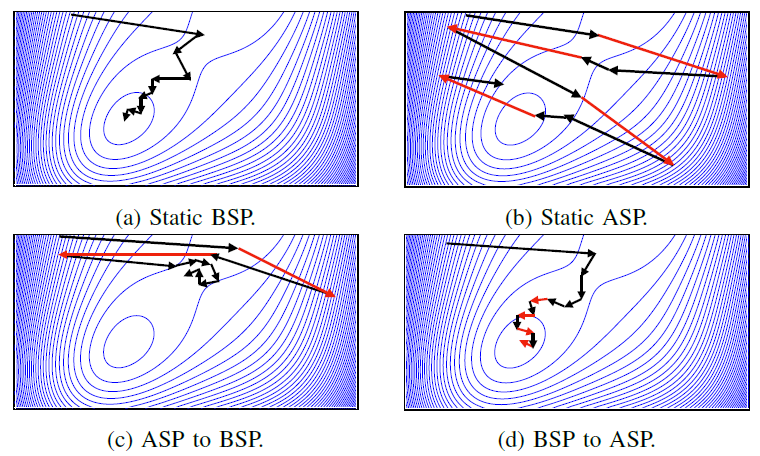
\includegraphics[scale=0.6]{P27.png}
		\caption{ترکیبات مختلف \lr{BSP} و \lr{ASP} بر روی یک تابع هزینه ساده \cite{Syncswitch2021}}
		\label{p27}
	\end{center}
\end{figure}

در الگوریتم گرادیان کاهشی تصادفی دسته‌ای \lr{(Minibatch SGD)} هر گره گرادیان را با استفاده از داده‌های محلی خودش محاسبه کرده و سپس گره‌ها گرادیان‌های محلی‌شان را میانگین می‌گیرند و از گرادیان حاصل برای به‌روزرسانی نهایی استفاده می‌شود. الگوریتم گرادیان کاهشی تصادفی محلی (\lr{Local SGD}) به عنوان بهبودی بر الگوریتم دسته‌ای پیشنهاد شده است. در این الگوریتم در هر دور هر گره \lr{K} گام از \lr{SGD} را بر روی هدف محلی و داده‌های خودش اجرا می‌کند. در نهایت نتایج به‌روزرسانی گره‌ها به عنوان نتیجه نهایی آن دور میانگین‌گیری می‌شود. در محیط‌های همکن و نزدیک به همگن نسخه محلی بر دسته‌ای غلبه می‌کند. در \cite{Minibatch2020} کارایی این دو نسخه در محیط‌های ناهمگن مورد بررسی قرار گرفته است. آنها نشان دادند که با تغییر تنظیمات از همگن به ناهمگن، کارایی نسخه محلی به طور قابل توجهی کاهش پیدا می‌کند. هر دوی این الگوریتم‌ها متمرکز می‌باشند.

همان‌طور که ذکر شد، الگوریتم گرادیان کاهشی تصادفی محلی برای همه سناریوها قابل اجرا نیست. گره‌ها ممکن است از نظر قابلیت‌های محاسباتی ناهمگن باشند و زمان مورد نیاز برای یادگیری محلی گره‌ها یکسان نیست. به همین دلیل یادگیری کاملا همگام گره‌ها ممکن است پرهزینه یا حتی غیرممکن باشد. اکثریت قریب به اتفاق کارهای ارائه شده یک مدل همگام استفاده می‌کنند که در آن همه گره‌ها قبل از ارسال به‌روزرسانی‌هایشان به سرور مرکزی، با تعداد تکرار یکسانی آموزش می‌بینند. همچنین در بیشتر کارهای انجام‌شده مدل ارتباطی \lr{Hub-and-Spoke} فرض می‌شود، اما این مدل بسیاری از حالت‌های دنیای واقعی را نشان نمی‌دهد. به عنوان مثال، دستگاه‌های موجود در یک شبکه اقتضایی متحرک به دلیل محدودیت‌های شبکه یا محدوده ارتباطی، ممکن است همه نتوانند در یک گام با سرور مرکزی ارتباط برقرار کنند. در چنین حالتی، یک مدل شبکه ارتباطی چند سطحی مناسب است. 

در \cite{zhou2019} الگوریتمی به نام \lr{SGD} محلی سلسله مراتبی \lr{ (HL-SGD)} برای یادگیری مدل در یک شبکه سلسله مراتبی با توپولوژی \lr{Hub-and-Spoke} پیشنهاد شده است و همه گره‌های شبکه همگن فرض شده‌اند. تحلیل خطا همگرایی و زمان همگرایی الگوریتم \lr{HL-SGD } در مقاله‌های \cite{Liu2020, Abad2020} برای یادگیری فدرالی \footnote{\lr{Federated Learning}} بحث شده است. الگوریتم \lr{SGD} محلی چندسطحی \lr{MLL-SGD} \cite{MLL2020} یک الگوریتم یادگیری توزیع‌شده برای شبکه‌های سلسله مراتبی با گره‌های ناهمگن است. در این الگوریتم، ساختار شبکه به صورت دو سطحی در نظر گرفته شده است. سطح پایین‌تر شامل مجموعه‌ای از شبکه‌های فرعی \lr{Hub-and-Spoke } است که هر کدام دارای یک سرور هاب و مجموعه‌ای از گره‌ها است. شبکه سطح بالا شامل یک شبکه هاب متصل که توسط آن هاب‌ها با هم ارتباط برقرار می‌کنند. هر شبکه فرعی چند دور \lr{SGD} محلی را اجرا می‌کند. بعد از یک دوره آموزش محلی گره‌ها، در مرکز شبکه فرعی میانگین‌گیری مدل انجام می‌شود. به طور دوره‌ای، هاب‌ها مدل‌های خود را با همسایگان در شبکه هاب میانگین‌گیری می‌کنند. در \cite{Fed6} پیشنهاد شده که از الگوریتم‌های بهینه‌سازی‌ غیر از \lr{SGD} در گره‌ها یا از یک قانون به‌روزرسانی جایگزین در سرور مرکزی استفاده شود. 

مکانیزم‌های کنترل مانع در الگوریتم‌های یادگیری تکراری نقش بسیار حیاتی را ایفا می‌کنند. در اغلب محاسبات داده-موازی، پارامترهای مدل اشتراکی براساس به‌روزرسانی‌های جداگانه از هر قطعه داده به‌روز می‌شوند. به عبارت دیگر، به‌روزرسانی‌های تجمیع‌شده برای به‌روزرسانی مدل استفاده می‌شوند. به‌روزرسانی‌های همگام نشده باعث ایجاد خطا و نویز در مدل نهایی خواهند شد. 

در یک محیط بسیار نامطمئن، لینک‌ها ممکن است خراب شوند و پهنای باند ناهمگن است؛ همچنین گره‌ها ثابت نیستند، می‌توانند در هر زمان به سیستم بپیوندند و یا از آن خارج شوند. بنابراین، در چنین محیطی با تضمین اینکه اکثر سیستم‌ها دارای مرز همگام‌شده هستند، می‌توان این تأثیرات را به حداقل رساند. میزان همگام‌سازی یک مانع نشان‌دهنده‌ی مبادله بین دقت (در هر تکرار) و کارایی (سرعت همگرایی) یک الگوریتم یادگیری تکراری است. با توجه به مزایا و معایب هر مکانیزم همگام‌سازی، \lr{BSP} قطعی است و می‌تواند به همان طراحی الگوریتم یادگیری ماشین منجر شود. مکانیزم‌های قطعی نظارت و کنترل همگام‌سازی مانع در یک محیط بسیار پویا ممکن است مناسب نباشند. در مقاله \cite{wang2017} یک تکنیک کنترل مانع احتمالی به نام \lr{PSP}\footnote{\lr{Probabilistic Synchronous Parallel}} بر اساس یک نمونه‌گیری اولیه ارائه شده است که در مقایسه با سه تکنیک کنترل مانع رایج در یک سیستم بسیار پویا و خیلی بزرگ به طور موثر سرعت همگرایی و مقیاس‌پذیری الگوریتم گرادیان کاهشی تصادفی را بهبود می‌بخشد. همگام‌سازی مانعی در تکنیک \lr{PSP} به روش احتمالی کنترل می‌شود، یعنی با نمونه‌برداری از گره‌های شرکت‌کننده در یادگیری درصدی از گره‌های سیستم که مرحله فعلی را به پایان رسانده‌اند را تخمین می‌زند. ایده اصلی مکانیزم \lr{PSP} این است که ما نیاز داریم که فقط بخشی از گره‌ها نه همه آنها، در پروسه همگام‌سازی قرار بگیرند. روش‌های موجود کنترل همگام‌سازی مانع و سازگاری مدل را تجمیع می‌کنند، درحالیکه \lr{PSP} کنترل همگام‌سازی مانع را از سازگاری مدل جدا می‌کند. 

در یادگیری فدرالی، گره‌های توزیع‌شده و ناهمگن برای یادگیری پارامترهای مدل با یکدیگر همکاری می‌کنند. با این‌حال، در حالی که مزایایی مانند حفظ حریم خصوصی با طراحی و کاهش تأخیر ایجاد می‌کند، شبکه ناهمگن چالش‌هایی را برای روش‌های همگام‌سازی یا روش‌های کنترل موانع، در مورد پیشرفت سیستم و همگرایی مدل و غیره ایجاد می‌کند. در \cite{Zhao2021} از مکانیزم \lr{PSP} برای یادگیری فدرال استفاده شده است و آنها پیشنهاد دادند که می‌توان مکانیزم‌های موجود، به ویژه \lr{BSP} و \lr{SSP}، را برای ایجاد مکانیزم‌های کنترل مانع کاملاً توزیع‌شده و مقیاس‌پذیرتر ترکیب کرد. این کار سبب می‌شود که با بزرگتر شدن سیستم به منظور جلوگیری از خفه شدن سرور و عدم ایجاد تنگنا، ارتباطات بین گره‌ها و سرور کاهش یابد. در شکل \ref{p28} مکانیزم احتمالی \lr{PSP} با \lr{BSP} ترکیب شده است و در نمونه‌برداری اولیه انجام شده از گره‌های موجود در سیستم، مکانیزم کنترل مانع \lr{BSP} اجرا شده است. 
\begin{figure}
	\begin{center}
		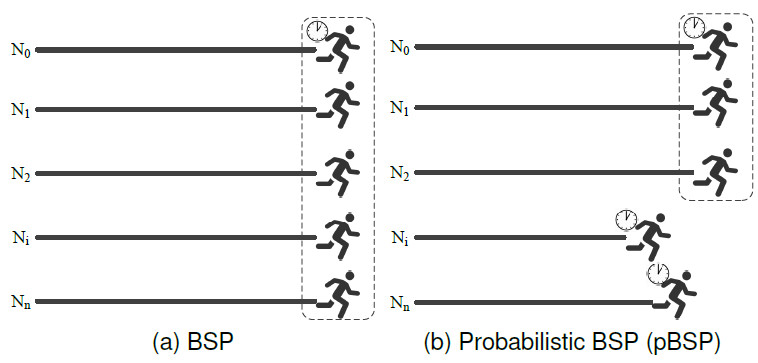
\includegraphics[scale=0.6]{P28.png}
		\caption{ترکیب \lr{PSP} با مکانیزم کنترل مانع \lr{BSP} \cite{wang2017}}
		\label{p28}
	\end{center}
\end{figure}

مقاله \cite{Fed9_2021} به بررسی فرصت‌های جدید یادگیری توزیع‌شده فدرالی برای سیستم‌های صنعتی شبکه‌ای نسل بعدی پرداخته است و مسائلی با تمرکز بر رانندگی مشارکتی در وسایل نقلیه خودکار متصل و روباتیک مشارکتی در تولید هوشمند مورد بحث قرار گرفته‌اند. راه‌حل‌های غیرمتمرکز پتانسیل بالایی برای نسل پنجم (\lr{5G}) صنعتی دارند. در مقاله \cite{Fed7_2021} رویکرد یادگیری توزیع‌شده غیرمتمرکزی مبتنی بر تبادل متقابل اجماع برای وسایل نقلیه خودکار متصل به منظور دسته‌بندی عوامل جاده ارائه شده است. عوامل جاده مانند عابران پیاده، مخروط‌های ترافیکی، موانع، دوچرخه‌ها، اتومبیل‌ها و اتوبوس‌ها  که هر وسیله نقلیه آن‌ها را با اسکن محیط از طریق خود توسط سنسور شناسایی می‌کند که در آن هدف وسایل نقلیه یادگیری مشارکتی یک مدل یادگیری عمیق مبتنی بر \lr{PointNet} برای استنباط نوع واقعی عوامل جاده است. 

برای رفع نیاز به همگام‌سازی دقیق در مکانیزم \lr{BSP} و کاهش زمان انتظار گره‌های سریع در مقاله \cite{zhao2020elastic} یک روش همگام‌سازی الاستیک یا قابل ارتجاع به نام \lr{ElasticBSP} پیشنهاد شده است. این روش همکام‌سازی مبتنی بر یک الگوریتم به نام \lr{ZipLine} است که زمان اجرای همگام‌سازی را تخمین می‌زند. در مرحله اول برای هر گره نقاط پایانی در تکرارهای آینده در زمان اجرا تخمین زده می‌شوند و در مرحله دوم یک الگوریتم تک-گذر بر روی نقاط پایانی تخمین زده شده‌ی همه گره‌ها اجرا می‌شود تا یک نقطه زمانی بهینه در تکرار بعدی برای همگام‌سازی به صورت سریع محاسبه گردد. 

هدف این روش تسهیل شرایط همگام‌سازی دقیق مکانیزم \lr{BSP} برای کاهش زمان انتظار گره‌ها و در نتیجه افزایش توان تکرارها، و در عین حال محدود کردن گرادیان‌های قدیمی و مقادیر قدیمی آنها در روند همگرایی الگوریتم گرادیان کاهشی تصادفی تکراری است. همچنین در مقایسه با مکانیزم \lr{SSP}، مدل پیشنهادی ظرفیت محاسباتی گره‌ها را در نظر می‌گیرد. بنابراین انعطاف‌پذیری و سازگاری بیشتری را در طول مرحله یادگیری بدون کاهش دقت مدل آموزشی، ارائه می‌دهد. 

در روش \lr{ElasticBSP}، زمان اعمال مانع همگام‌سازی متفاوت است و هر ابرگام تعداد متفاوتی از تکرارها را برای هر گره مجاز می‌کند. این مقادیر در زمان اجرا توسط الگوریتم \lr{ZipLine} تعیین می‌شوند که حداقل زمان انتظار کلی همه گره‌ها را به دست می‌آورد. شکل \ref{p2930} به خوبی تفاوت زمان اجرای ابرگام‌ها در \lr{BSP} و \lr{ElasticBSP}  در یک شبکه با 4 گره را نشان می‌دهد. در هر ابرگام قسمت رنگی هر گره زمان محاسبات و قسمت سفید رنگ زمان ارتباطات را بیان می‌کنند.
%\iffalse
\begin{figure}
	\centering
	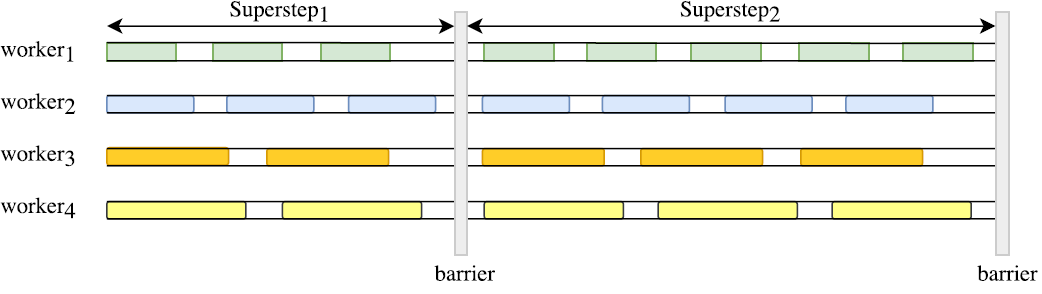
\includegraphics[width=\textwidth]{Pic29.png}
	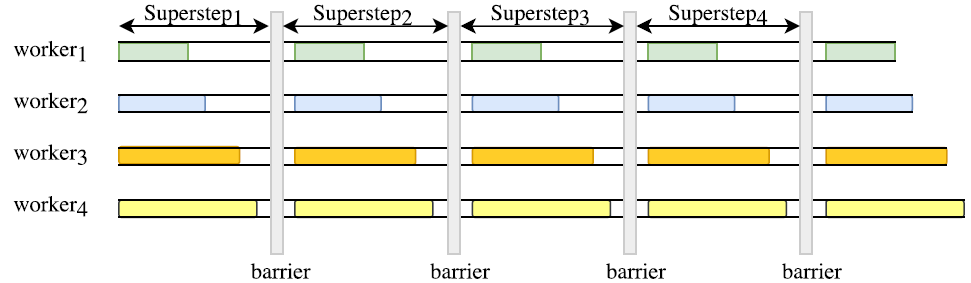
\includegraphics[width=\textwidth]{Pic30.png}
	\caption{تفاوت زمان اجرای ابرگام‌ها در \lr{BSP} و \lr{ElasticBSP} \cite{Zip2021}}
	\label{p2930}
\end{figure}







\subsection{الگوریتم‌های یادگیری تطبیقی انتشاری}\label{DfsnAlg}


الگوریتم‌های یادگیری تطبیقی انتشاری بر اساس پردازش داده و همکاری‌ها بین گره‌ها پایه‌ریزی شده‌اند و هر گره با استفاده از داده‌هایی که در اختیارش می‌باشد، تخمینی از پارامترهای مجهول ارائه می‌دهد و می‌تواند با توجه به توپولوژی شبکه با همسایه‌هایش تعامل داشته باشد و از آن‌ها اطلاعات دریافت کند و به آن‌ها نیز اطلاعاتی ارسال نماید. بنابراین، پردازش انجام شده مبتنی‌بر داده‌های محلی هر گره و اطلاعات دریافتی از همسایه‌هایش می‌باشد. بر خلاف روش تخمین پارامتر متمرکز، در این روش هیچ گره مرکزی وجود ندارد و قادر است سربار ارتباطی و پردازشی را کاهش دهد. اکثر کارهای ارائه‌شده در زمینه برآورد پارامتر از طریق شبکه‌های تطبیقی توزیع‌شده به صورت یک مساله کمینه‌سازی اجماع توابع هزینه هر گره مطرح می‌شوند. گره‌ها با توابع زیان مجزا اما هم مدل در جستجوی یک هدف مشترک هستند و نیاز به همگرا شدن به سمت یک پارامتر مشترک دارند. این مسائل تک‌وظیفه‌ای نامیده می‌شوند. 

در شکل \ref{p11} دسته‌بندی الگوریتم‌های یادگیری تطبیقی انتشار برای مقابله با چالش‌های موجود در شبکه‌های تطبیقی توزیع‌شده نشان داده شده است. این دسته‌بندی براساس سه دیدگاه انجام شده است: الف) تک وظیفه‌ای و چندوظیفه‌ای ب) روش‌های همگام و غیرهمگام ج) تابع هدف. جزییات این الگوریتم‌ها در ادامه همین بخش بیان شده است. در دسته‌بندی انجام شده شکل \ref{p11}، الگوریتم‌های یادگیری انتشاری پیشنهادی در این رساله به منظور مشخص شدن جایگاه شان نیز آورده شده‌اند. 

\begin{figure}
	\begin{center}
		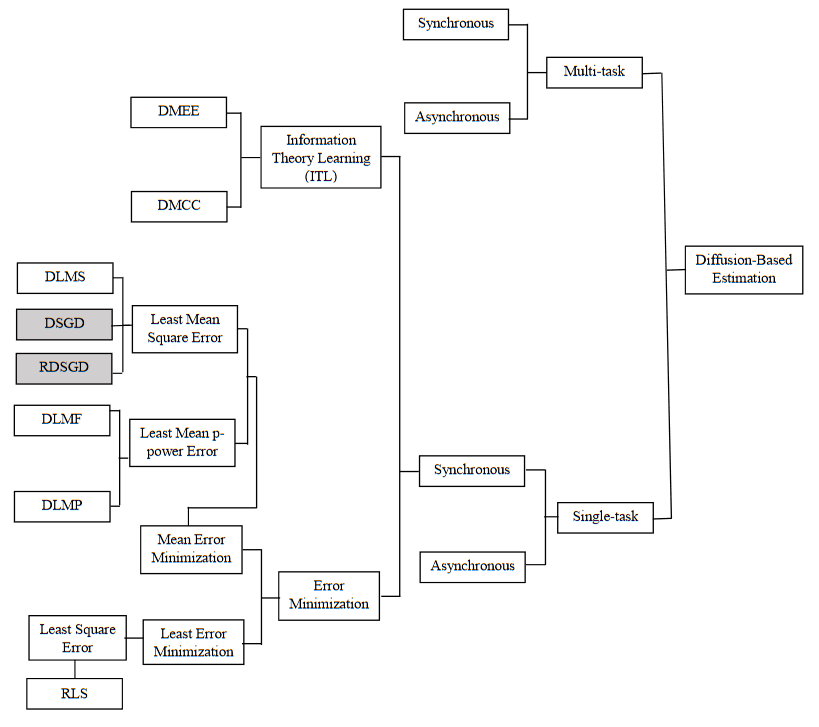
\includegraphics[scale=1.2]{CatDiffusion__.PNG}
		\caption{دسته‌بندی الگوریتم‌های یادگیری تطبیقی انتشار}
		\label{p11}
	\end{center}
\end{figure}

در مقاله \cite{Lop2008} الگوریتم \lr{DLMS} که مبتنی بر روش همکاری انتشار می‌باشد از استراتژی تطبیق سپس ترکیب \lr{ATC }\footnote{\lr{Adapt Then Combine (ATC)}} يا تركيب سپس تطبيق  \lr{CTA} \footnote{\lr{Combine Then Adapt (CTA)}} برای حل رابطه بهینه‌سازی \ref{e1} استفاده می‌کند. روابط زیر فرم به‌روزرسانی کلی \lr{ATC} برای هر گره $k$ را نشان می‌دهند.

\begin{equation}\label{ATC1}
	\begin{cases}
		\psi_{k}(i+1)=w_{k}(i)-\mu_k\sum_{l\in N_k}c_{lk}\nabla_{w}{J_l(w_{k}(l))}\quad\text{(\lr{Adapt})}\\
		w_{k}(i+1)=\sum_{l\in N_k}a_{lk}\psi_{l}(i+1) \quad  \text{(\lr{Combine})}
	\end{cases}
\end{equation}

همچنين روابط فرم به‌روزرسانی کلی \lr{CTA} برای هر گره $k$ به صورت زير بيان مي‌شوند:
\begin{equation}\label{CTA1}
	\begin{cases}
		\psi_{k}(i)=\sum_{l\in N_k}a_{lk}w_{l}(i)\quad  \text{(\lr{Combine})}\\
		w_{k}(i+1)=\psi_{k}(i)-\mu_k\sum_{l\in N_k}c_{lk} \nabla_{w}{J_l(\psi_{k}(i))}\quad\text{(\lr{Adapt})}
	\end{cases}
\end{equation}
که ${J_l(\psi_{k}(i))}$ تخمین بردار گرادیان گره $l$ می‌باشد و $\mu_k$ ضریب همگرایی و $c_{lk}$ و $a_{lk}$ ضرایب غیرمنفی هستند که براساس شرایط زیر تعریف می‌گردند:
\begin{equation}\label{e8}
	a_{lk}>=0,\qquad\sum_{l\in N_k}a_{lk}=1, \qquad and\quad a_{lk}=0 \quad if \quad  l\notin N_k
\end{equation}

\begin{equation}\label{e9}
	c_{kl}>=0, \qquad \sum_{l\in N_k}c_{kl}=1,\qquad and\quad c_{kl}=0\quad if \quad l\notin N_k 
\end{equation}

طبق شرط‌های ذکر شده برای ضرایب $c_{lk} $ و $a_{lk}$ با جمع‌آوری آنها در یک ماتریس  \lr{N*N} دو ماتریس ترکیبی وزن‌دار $A=[a_{lk}]$ و $C=[c_{lk}] $ به صورت $1C=1$ و $1A^T=1$ تعریف می‌شوند. روش‌های متعددی برای انتخاب ضرایب وزن همسایگی $a_{lk}$ بین دو گره در شبکه ارائه شده است. یکی از ساده‌ترین روش‌ها براساس تعداد گره‌های همسایه است که به صورت زیر تعریف می‌شود:

\begin{equation}\label{e10}
	a_{lk}=
	\begin{cases}
		\frac{1}{|N_k|} \quad  l\in N_k\\
		0 \quad l\notin N_k
	\end{cases}
\end{equation}
در شکل \ref{p7} روش‌های دیگری که برای انتخاب ضرایب $a_{kl} $ استفاده می‌شوند، ذکر شده است.
\begin{figure}
	\begin{center}
		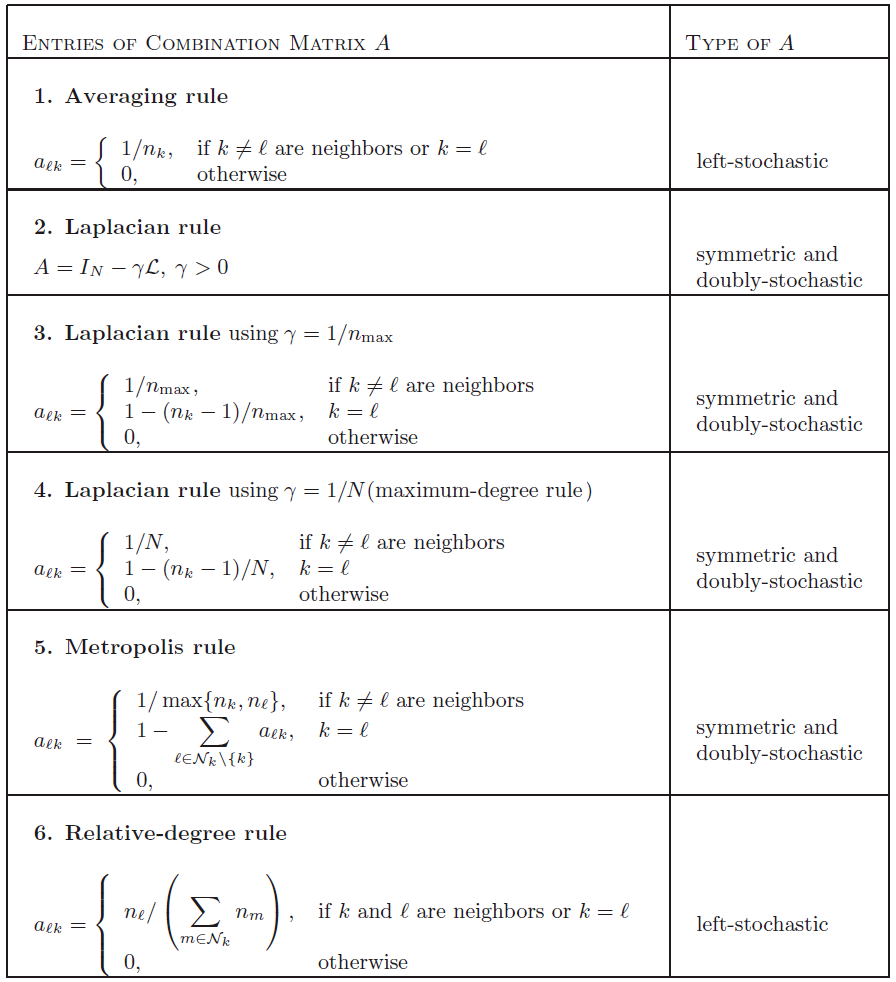
\includegraphics[scale=0.6]{Pic7.png}
		\caption{روش‌های مختلف تعریف ضرایب وزن همسایگی  \cite{SayedBook}}
		\label{p7}
	\end{center}
\end{figure}

شکل \ref{p8} استراتژی \lr{ATC} را در شبکه‌های تطبیقی توزیع‌شده با روش انتشار نشان می‌دهد. همان طور که دیده می‌شود، هر گره $k$ ابتدا با استفاده از فیلتر وفقی خود به‌روزرسانی بردار پارامتر میانی را انجام می‌دهد و سپس بردارهای پارامتر میانی همسایگان را ترکیب می‌نماید.
\begin{figure}
	\begin{center}
		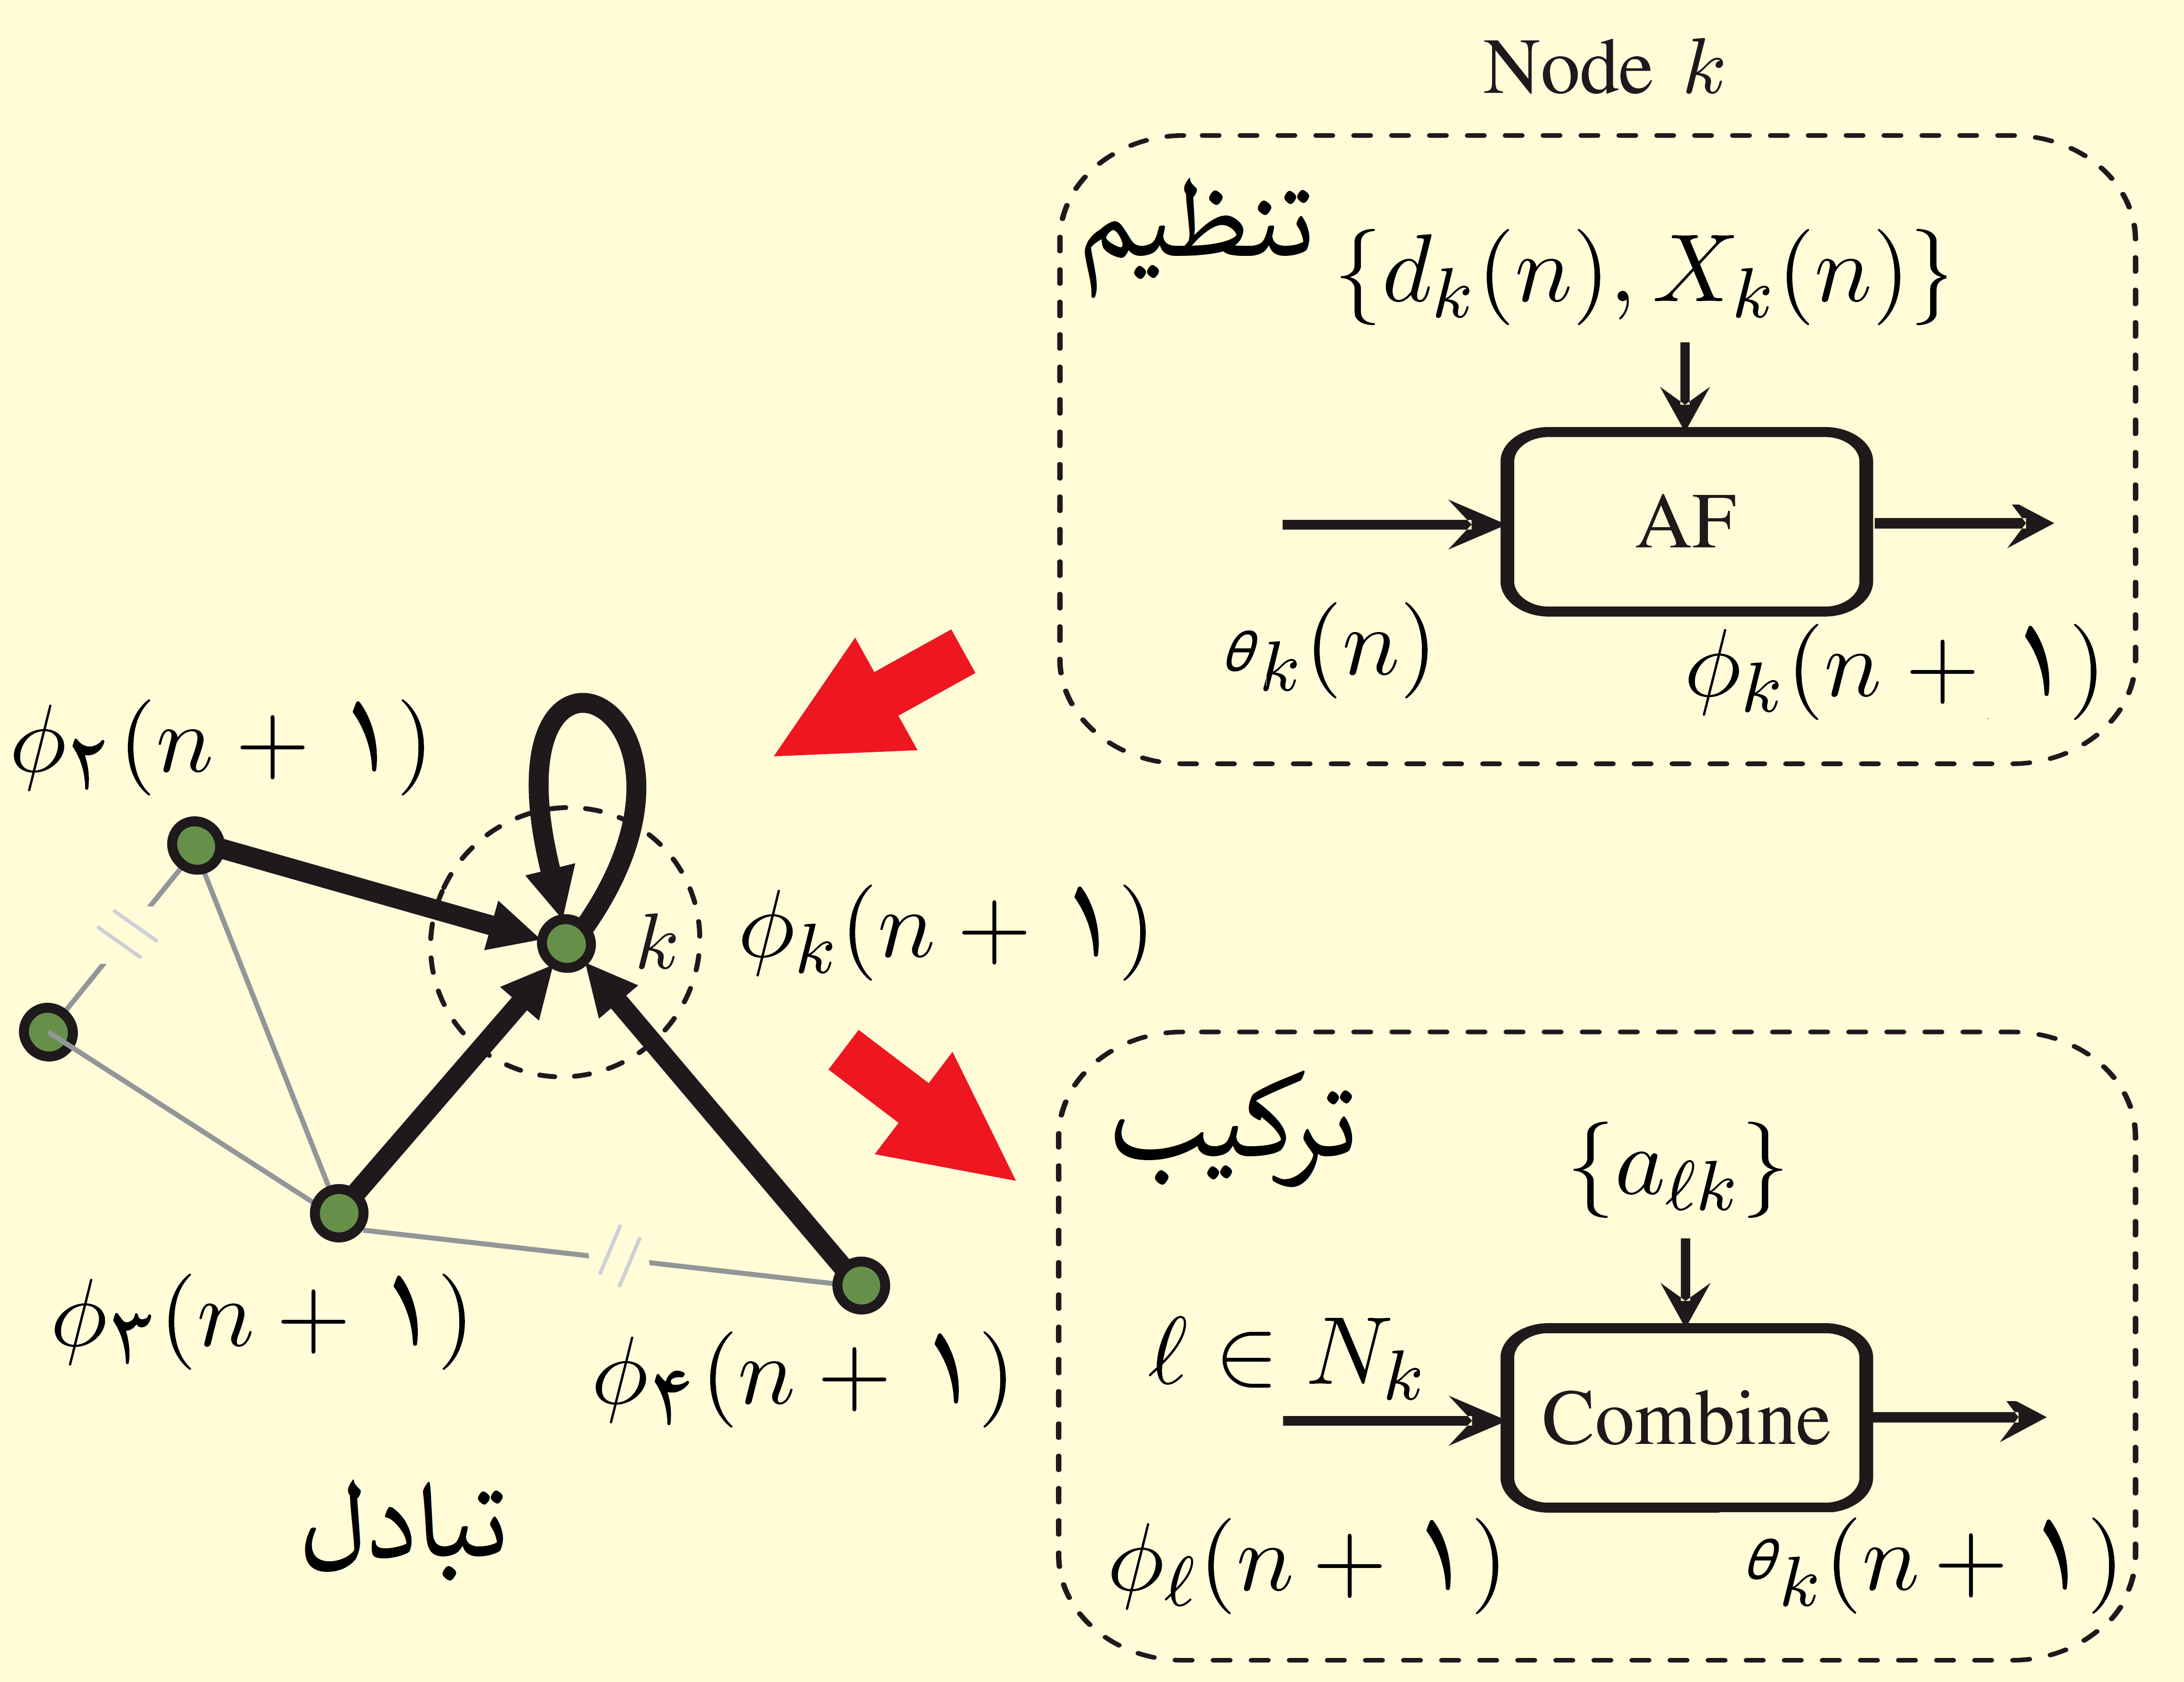
\includegraphics[scale=0.07]{Pic8.JPG}
		\caption{استراتژی \lr{ATC} در شبکه‌ تطبیقی انتشاری  \cite{SayedBook}}
		\label{p8}
	\end{center}
\end{figure}
در استراتژی تركيب سپس تطبيق يا همان \lr{CTA} ابتدا تخمين مياني با تركيب تخمين‌هاي محلي گره‌هاي همسايه محاسبه مي‌گردد. سپس با استفاده‌ از داده‌هاي محلي گره $k$ و تخمين مياني بدست آمده از گام اول، عمليات تطبيق انجام مي‌شود. شکل \ref{p9} استراتژی \lr{CTA} را در شبکه‌های تطبیقی توزیع‌شده با روش انتشار نشان می‌دهد.

\begin{figure}
	\begin{center}
		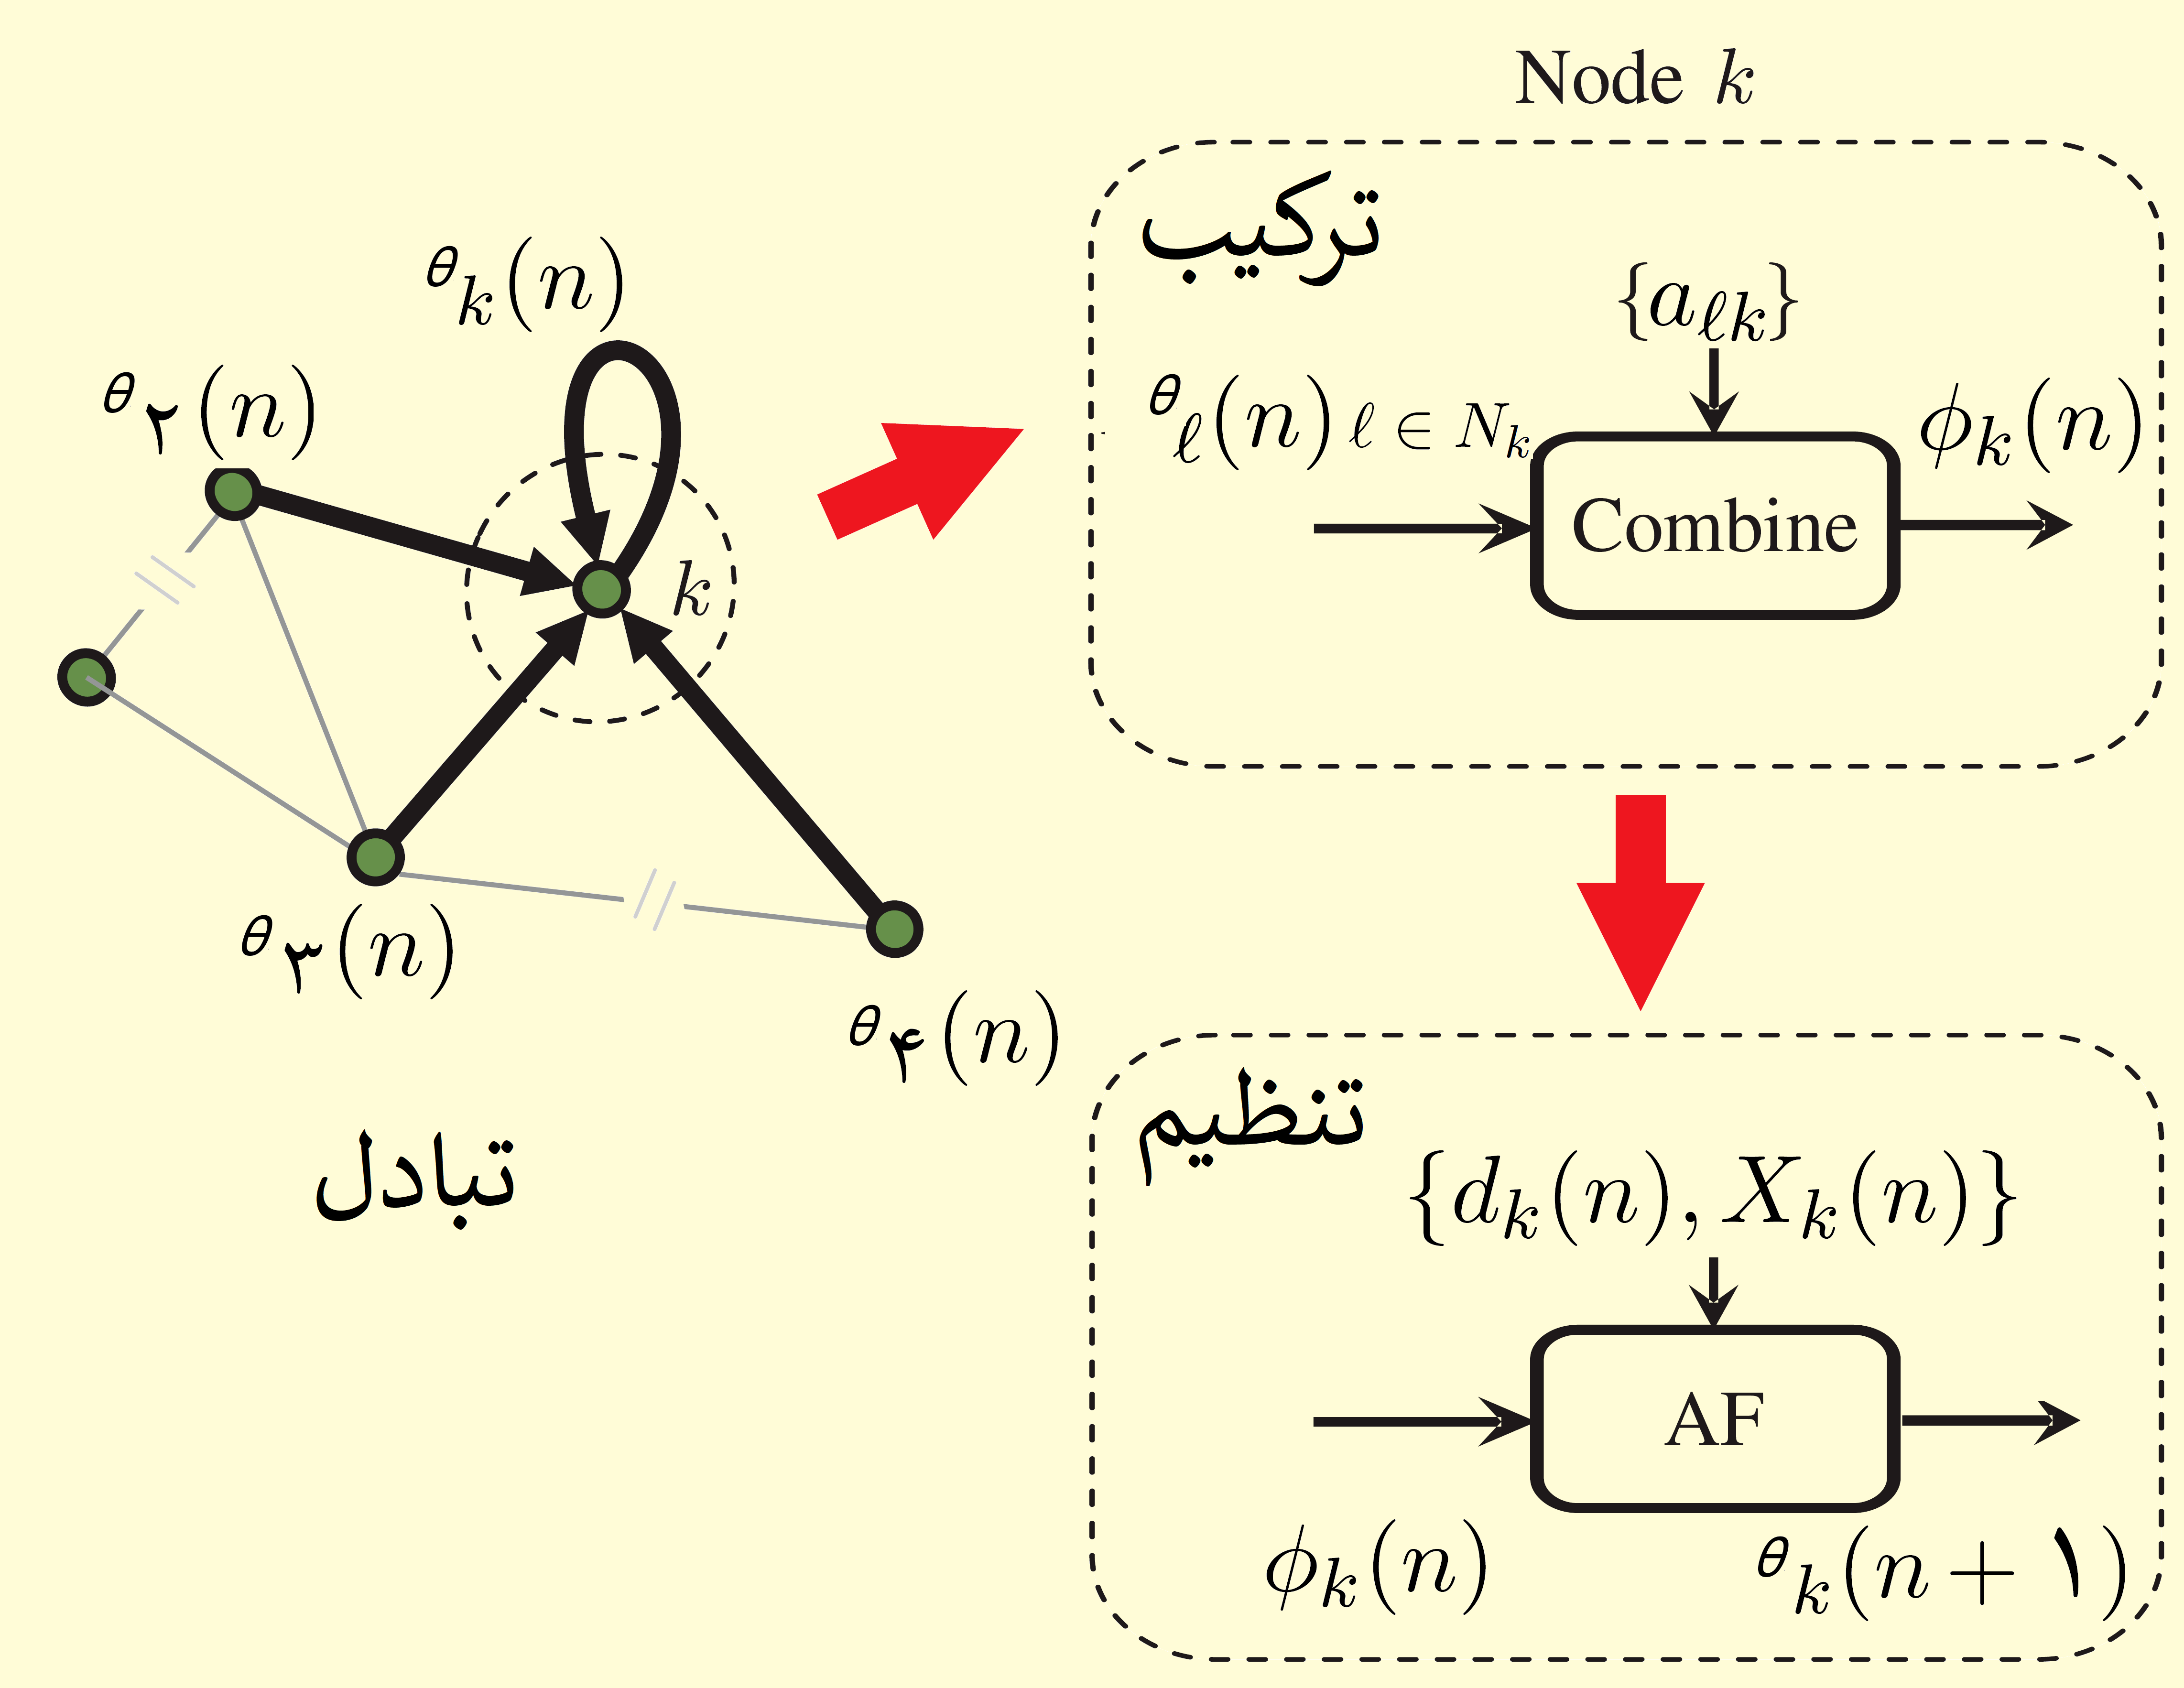
\includegraphics[scale=0.07]{Pic9.JPG}
		\caption{استراتژی \lr{CTA} در شبکه‌ تطبیقی انتشاری  \cite{SayedBook}}
		\label{p9}
	\end{center}
\end{figure}


سایر روش‌های ارائه شده برای حل \lr{DLMS} از جمله استراتژی \lr{ATC} بدون تبادل اطلاعات بین گره‌های همسایه در مرحله تطبیق، استراتژی ترکیب سپس تطبیق \lr{CTA} بدون تبادل اطلاعات در شکل \ref{p10} لیست شده‌اند \cite{Cat20081}. 

\begin{figure}
	\begin{center}
		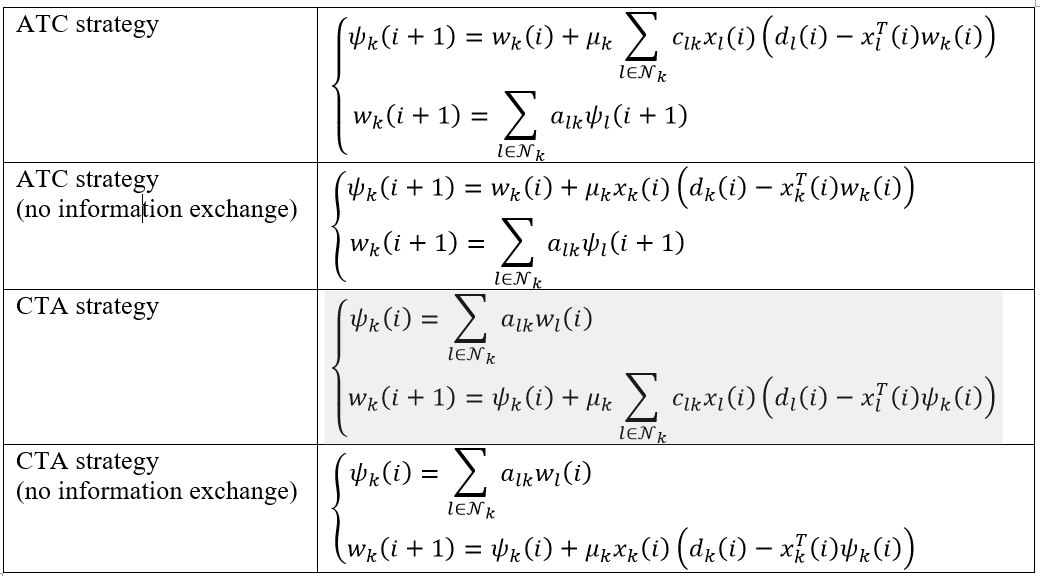
\includegraphics[scale=0.8]{Pic10.JPG}
		\caption{: روش‌های مختلف حل \lr{DLMS}   \cite{Cat20081}}
		\label{p10}
	\end{center}
\end{figure}

در مقاله \cite{Cat20082} با استفاده از فيلتر \lr{RLS} الگوریتم یادگیری توزیع‌شده انتشاري به نام \lr{DRLS} ارائه شده است. با فرض مدل شدن ورودي‌هاي فيلتر با رگرسيون خطي بيان‌شده در رابطه \ref{e6} و تعريف ماتريس‌هاي \lr{A} و \lr{C} همانند الگوریتم \lr{DLMS}، مساله بهينه‌سازي زير با ترم تنظيم $\delta$  و ضريب فراموشي $\lambda$\footnote{\lr{Forgetting factor}}  به منظور تخمين بردار پارامتر $w^o$ استفاده مي‌شود:

\begin{equation}\label{e13}
	\min_w \lambda^{i+1}\delta ||w||^2 +\sum_{l=0}^{i}\lambda^{i-j}(\sum_{k=1}^{N}(d_k(i)-u_k^T(i)w)^2)
\end{equation}

كه $\delta>0$ و  ضریب فراموشي $0\le\lambda\le1$ است. حل مساله بهينه‌سازي بيان شده در رابطه \ref{e1} بر اساس استراتژي \lr{ATC} در ادامه آورده شده است. براي هر گره $k$، مقادير اوليه زير در نظر گرفته مي‌شود:

\begin{equation}\label{e14}
	\begin{cases}
		w_{k,-1}=0,\quad P_{k,-1}=\delta^{-1}I_M\\
		\psi_{k,i}=w_{k,i-1}\\
		P_{k,i}=\lambda^{-1}P_{k,i-1}
	\end{cases}
\end{equation}

براي هر گره $k$ روابط گام تطبيق با تكرار بر روي همه همسايگان $l\in N_k$ و گام تركيب اين رويكرد به صورت زير بيان مي‌شوند:

\begin{equation}\label{e141}
	\begin{cases}
		\begin{cases}
			\psi_{k,i}=\psi_{k,i}+\frac{c_{lk}P_{k,i}u_{l,i}^T}{1+c_{lk}u_{l,i}P_{k,i}u_{l,i}^T}\left[d_{l,i}-u_{l,i}\psi_{k,i}\right]\\
			P_{k,i}=P_{k,i}-\frac{c_{lk}P_{k,i}u_{l,i}^T u_{l,i}P_{k,i}}{1+c_{lk}u_{l,i}P_{k,i}u_{l,i}^T}
		\end{cases}\quad  \text{(\lr{Adapt})}\\
		w_{k,i}=\sum_{l\in N_k}a_{lk}\psi_{l,i}\quad  \text{(\lr{Combine})}
	\end{cases}
\end{equation}

در مقاله\cite{Jung2013} روشي براي جبران باياس بر اساس نسخه نرمال \lr{LMS} ارائه شده است تا بتواند اثر منفي نويز ورودي را كاهش دهد. براي حذف باياس نويز ورودي از معياري استفاده شده كه نيازمند تخمين واريانس نويز ورودي است. اما زمانيكه نويز ضربه‌اي باشد، تخمين واريانس نويز چندان موفقيت‌آميز نمي‌باشد. بنابراين براي حل اين مشكل، تخمين واريانس نويز ورودي زمان رخ دادن نويز ضربه‌اي به‌روز خواهد شد. اگر خطا از يك حد مشخصي بيشتر شود، واريانس نويز ورودي مجدد تخمين‌زده مي‌شود و سپس مقدار بردار پارامتر به‌روزرساني مي‌شود. در مقاله \cite{Zheng2017} از الگوريتم حداقل توان چهارم خطا براي بدست آوردن تخميني بدون باياس استفاده شده است. 

\begin{figure}
	\begin{center}
		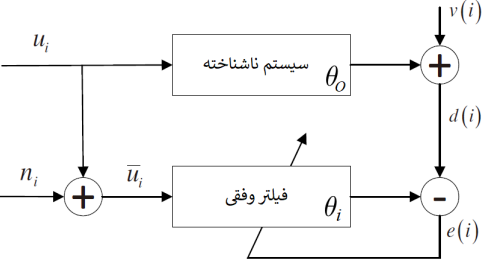
\includegraphics[scale=0.9]{Filter.png}
		\caption{فیلتر تطبيقي با نويز ورودي}
		\label{filter}
	\end{center}
\end{figure}

در شبكه‌هاي تطبيقي توزيع‌شده براي مقابله با مساله نويز ورودي روش‌هايي مختلفی ارائه شده است. شكل \ref{p24} اين مساله را در شبكه‌هاي تطبيقي نشان مي‌دهد. در مقاله \cite{Abdolee2016} روشي بر اساس تخمين واريانس نويز پيشنهاد داده‌اند كه تابع هدف هر گره \lr{k} به صورت زير تعريف مي‌شود:
\begin{equation}\label{e142}
	J_k(w)=E\lvert\lvert d_k(i)-u_{k,i}w\rvert\rvert^2-\sigma^2_{k,i}\lvert\lvert w \rvert\rvert^2
\end{equation}


كه $\sigma_{k,i}^2$ واريانس نويز ورودي در گره $k$ام شبكه است. از الگوريتم انتشار براي حل اين مساله بهينه‌سازي استفاده مي‌شود و روابط به‌روزرساني به‌دست مي‌آيد. اين روش نيازمند تخمين واريانس نويز ورودي است. برخي از كارهاي ارائه شده از توابع زيان پايدارتري براي مقابله با نويز‌هاي ورودي كمك مي‌گيرند. 

\begin{figure}
	\begin{center}
		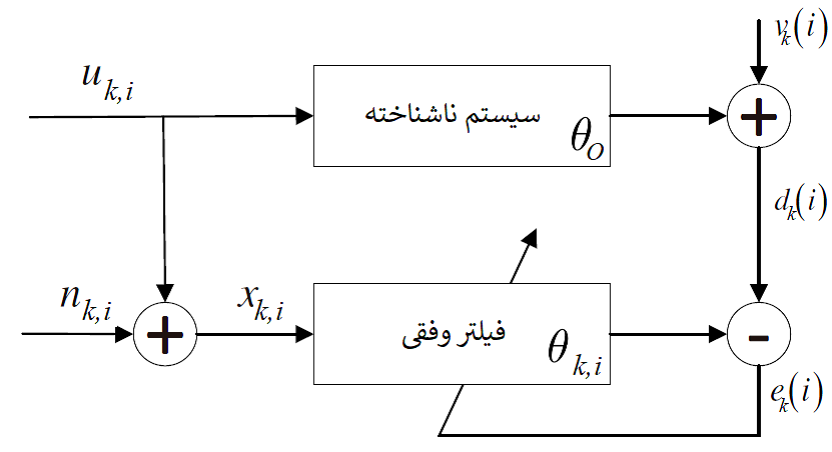
\includegraphics[scale=0.6]{Pic24.png}
		\caption{شبكه تطبيقي با نويز ورودي  \cite{Abdolee2016}}
		\label{p24}
	\end{center}
\end{figure}
در \cite{Naeimi2024_RClass} به منظور مقاوم‌سازی طبقه‌بندی آنلاین  با استفاده از روش یادگیری توزیع‌شده انتشاری از یک تابع خطا کسینوس لگاریتمی مشتق‌شده استفاده شده است  که برای نویزهای ضربه‌ای مناسب است.

حذف یا کاهش نویز و تداخل سیگنال صوتی یک فناوری پیشرفته است که امروزه  به منظور کاهش یا حذف صداهای ناخواسته و مزاحم در محیط‌های مختلف به کار میرود و یک چالش مهم در پردازش سیگنال می‌باشد. محققان روش‌های مختلفی از جمله روش‌های مبتنی بر فیلترهای تطبیقی ​​را برای رفع این مشکل معرفی کرده‌اند. در مقاله \cite{Bahraini2024_NoiseCncl} یک \lr{RLS} مقاوم مبتنی بر فیلتر تطبیقی با لگاریتم طبیعی و یک تابع خطا کسینوس هذلولی ارئه شده است که روشی را برای حذف نویز صوتی در برابر انواع خاصی از نویزها فراهم می‌کند. 

كارهاي انجام شده در زمينه مقاوم‌سازي رويكرد‌هاي توزيع‌شده مبتني بر انتشار در برابر نويز را با توجه به تابع هدف مي‌توان به دو دسته الگوريتم‌هاي مبتني بر حداقل‌سازي ميانگين مربعات خطا (\lr{MSE}) و الگوريتم‌هاي مبتني بر مفاهيم تئوري اطلاعات (\lr{ITL}) تقسيم كرد. اگر نويز موجود از مدل گوسي باشد، الگوريتم‌هاي مبتني بر حداقل‌سازي ميانگين مربعات خطا كه به واريانس نويز وابسته هستند، كارآيي مناسبي دارند. اما در برابر نويز غيرگوسي عملكرد مناسبي ندارند و در بعضی مواقع واگرا نيز مي‌شوند. به همين دليل، كارهايي ارائه شده است كه با جايگزين كردن \lr{MSE} با توابع هزينه مقاوم‌تر سعي بر مقابله با نويز‌هاي غيرگوسي دارند. در مقاله \cite{Li2013} الگوريتم حداقل آنتروپي خطا كه يكي از الگوريتم‌هاي مبتني بر تئوري اطلاعات است، بدين منظور استفاده شده است و در آن آنتروپي آخرين \lr{N} نمونه‌اي كه بيشترين ميزان خطا را دارند، به عنوان تابع هدف براي حداقل نمودن خطا استفاده مي‌شود. الگوريتم انتشار معيار حداكثرسازي کورآنتروپی (\lr{DMCC}) \cite{MA2016} از كرنل گوسي به دليل توانايي آن در رد كردن نمونه‌هاي آغشته به نويز غيرگوسي استفاده شده است. تابع هدف اين الگوريتم به صورت زير تعريف مي‌شود:
\begin{equation}\label{e143}
	\begin{cases}
		J_k^{local}(w)=\sum_{l\in N_k}c_{lk} G_{\sigma}(e^2_{l,k})\\
		G_{\sigma}(e^2_{l,k})=\frac{1}{\sigma \sqrt{2\pi}}\exp(-\frac{1}{2\sigma^2}(d_{l,i}-u_{l,i}w_l)^2)
	\end{cases}
\end{equation}

كه $G_{\sigma}(e^2_{l,k})$ تابع استاندارد گوسي با عرض كرنل $\sigma$ است.

الگوريتم‌هاي مبتني بر حداقل‌سازي ميانگين مربعات خطا با تغيير دادن تابع هدف سعي در مقاوم‌سازي در برابر نويز غيرگوسي دارند. الگوريتم انتشار علامت خطا \lr{DSignLMS} \cite{Ni2016} از علامت خطا در تابع هدف استفاده مي‌شود:
\begin{equation}\label{e144}
	\begin{cases}
		J_k^{local}(w)=\sum_{l\in N_k}c_{lk} \lvert\lvert e_{l,k}\rvert\rvert_1\\
		s.t. \lvert\lvert \phi_{k,i}-\theta_{k,i-1}\rvert\rvert^2_2\le\mu_k^2
	\end{cases}
\end{equation}

كه $\phi_{k,i}$ تخمين مياني در گره‌ $k$ام است و بردار گراديان اين الگوريتم به صورت $\nabla J_k^{local}(w)=\sum_{l\in N_k}c_{lk}u_{l,k}sgn(e_{l,k})$ محاسبه مي‌شود. 

در الگوريتم انتشار  \lr{DLMF} \cite{Park2014} ميانگين توان چهارم خطا در تابع هدف براي مقابله با نويز غيرگوسي به كارگرفته شده است. همچنين در الگوريتم انتشار \lr{RDLMS} \cite{Ashk} از تابع زيان شبه‌هابر\footnote{\lr{Pseudo-huber}} بدين منظور استفاده شده است. در \cite{Bert2011} روش‌هايي براي مقابله با داده‌هاي نويزي در الگوريتم \lr{RLS} مطرح شده است و همچنین در \cite{Naeimi2024_GMBZ} با معرفی تابع زیان جدیدی به نام \lr{GMBZ} به منظور مقاوم‌سازی در برابر نویزهای غیرگاوسی و کاهش تعدیل نادرست در حالت پایدار، الگوریتم مقاوم \lr{RLS} مبتنی بر تابع زیان \lr{GMBZ} ارائه داده‌اند. 

الگوريتم‌ها و رويكرد‌هايي كه تاكنون براي شبكه‌هاي تطبيقي توزيع‌شده مطرح‌شده‌‌اند، با فرض داشتن محیط همگام عمل مي‌كردند. با در نظر گرفتن اتفاقات تصادفي همچون زمان ورود داده‌ها، خرابي گره‌ها و لينك‌ها، تغييرات توپولوژي شبكه و غیره، در مقاله \cite{Zhao2014} پياده‌سازي الگوريتم انتشار با رويكرد \lr{ATC} به صورت زير در محيط غیرهمگام ارائه شده است.
\begin{equation}\label{e145}
	\begin{cases}
		\psi_k(i)=w_k(i-1)-\mu_k(i) \nabla_{w^T}J_k({w_k(i-1)})\qquad(Adapt)\\
		w_k(i)=\sum_{l\in N_{k,i}}a_{lk}(i)\psi_l(i)\qquad(Combine)
	\end{cases}
\end{equation}
كه در رويكرد غیرهمگام، پارامترهای $\mu_k(i)$ و $a_{lk} (i)$ با زمان تغییر می‌کنند و $N_{k,i}$ مجموعه همسایگی گره $k$ در زمان $i$ را بیان می‌کند. 

\subsection{نقاط ضعف روش‌های موجود}
به طور کلی، تمامی راه‌کارهایی که از روش‌های موجود استفاده می‌کنند شامل نقاط ضعف یکسانی می‌باشند. شکل \ref{Disadvantage} نقاط ضعف تمامی راه‌کار‌ها را با توجه به روش مورد استفاده نشان می‌دهد. 
 
\begin{figure}
	\begin{center}
		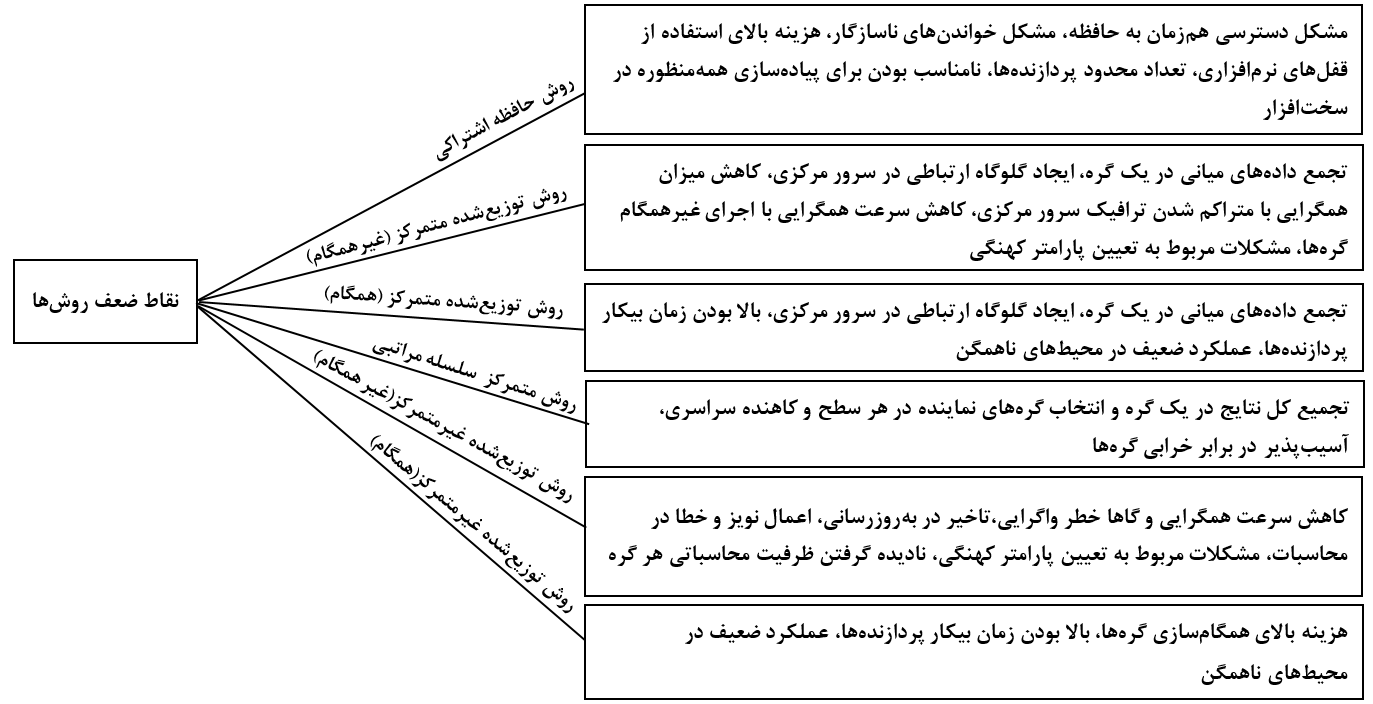
\includegraphics[scale=0.7]{DisAd_.PNG}
		\caption{بیان نقاط ضعف راه‌کارهای موجود}
		\label{Disadvantage}
	\end{center}
\end{figure}

روش‌های حافظه اشتراکی و حافظه اشتراکی توزیع‌شده همانند ماشین‌های \lr{NUMA} از مشکلات بسیاری رنج می‌برند، از جمله 1) محدود بودن تعداد پردازنده‌ها، 2) عدم مناسب بودن برای پیاده‌سازی‌های همه منظوره در سخت‌افزار و همچنین 3) دسترسی هم‌زمان پردازنده‌ها به حافظه اشتراکی و 4) عملیات خواندن ناسازگار. در برخی از تحقیقات به منظور همگام‌سازی پردازنده‌ها و جلوگیری از رخ دادن مشکلات ذکر شده، از قفل‌های نرم‌افزاری استفاده شده است که این قفل‌ها هزینه بالایی را متحمل می‌کنند. 

روش‌های توزیع‌شده یا شبکه‌های کامپیوتری متمرکز به دلیل استفاده از سرورهای مرکزی درگیر مشکلاتی از جمله تجمع داده‌های میانی در یک یا چند گره مرکزی، ایجاد گلوگاه ارتباطی، شلوغ شدن بار ترافیکی در سرورهای مرکزی و کاهش میزان همگرایی با متراکم شدن ترافیک در سرور مرکزی، می‌باشند. در صورتی که روش‌های توزیع‌شده متمرکز به صورت غیرهمگام اجرا شوند، شامل نقاط ضعف کاهش سرعت همگرایی با اجرای غیرهمگام  و تعیین پارامتر کهنگی خواهند بود. در مقابل روش‌های توزیع‌شده متمرکز همگام از نقاط ضعف بالا بودن زمان بیکاری گره‌ها و عملکرد ضعیف در محیط‌های اجرایی ناهمگن رنج می‌برند. 

روش‌های توزیع‌شده متمرکز سلسله مراتبی که از یک ساختار کلاینت-سرور چند سطحی استفاده می‌کنند، شامل نقاط ضعفی همانند انتخاب گره‌های نماینده در هر سطح و انتخاب کاهنده‌ سراسری و آسیب ‌پذیری در برابر خرابی گره‌ها و یال‌ها می‌باشند. 

روش‌های توزیع‌شده غیرمتمرکز دیگر درگیر مشکلاتی از جمله گلوگاه شدن سرور مرکزی و کاهش میزان همگرایی با متراکم شده ترافیک در سرور مرکزی و آسیب پذیری در برابر خرابی گره‌ها و یال‌ها، نیستند. اما اگر این روش‌ها به صورت غیرهمگام اجرا شوند، متحمل مشکلاتی از جمله کاهش سرعت همگرایی به دلیل استفاده از داده‌های غیرهمگام تبادل‌شده توسط پردازنده‌ها، تعیین پارامتر کهنگی  به منظور جلوگیری از کاهش سرعت همگرایی پردازنده‌ها، اعمال نویز و خطا در محاسبات پردازنده‌ها به دلیل استفاده از داده‌های کهنه و غیرهمگام و همچنین در نظر نگرفتن ظرفیت محاسباتی پردازنده‌ها در عملیات یادگیری، می‌باشند. روش‌های توزیع‌شده غیرمتمرکز همگام نیز با مشکلات خاص خود درگیر می‌باشند. هزینه بالای همگام‌سازی پردازنده‌ها با یکدیگر، بالا بودن زمان انتظار و بیکاری آنها و همچنین عملکرد ضعیف در محیط‌های اجرایی ناهمگن برخی از این مشکلات می‌باشند.  


\section{خلاصه}
در این فصل مطالعاتی در مورد نحوه اجرای روش‌های یادگیری توزیع‌شده بر روی سیستم‌های حافظه اشتراکی و سیستم‌های حافظه توزیع‌شده انجام شده است. این مطالعات با توجه به راه‌حل‌هایی که وجود داشت به دو بخش تقسیم شده‌اند. بخش اول مربوط به راه‌حل‌هایی است که یادگیری توزیع‌شده را بدون هیچ مدل محاسباتی انجام داده‌اند. در بخش دوم راه‌حل‌های یادگیری توزیع‌شده مبتنی بر مدل محاسباتی و پژوهش‌های انجام شده در این زمینه مورد مطالعه و بررسی گرفته است. سپس نقاط ضعف هر یک از روش‌ها به صورت خلاصه بیان شده است. در انتها، الگوریتم‌های یادگیری توزیع‌شده انتشاری موجود به عنوان الگوریتم یادگیری مورد استفاده در شبکه‌های تطبیقی توزیع‌شده مورد بررسی و مطالعه قرار گرفتند. 




